\chapter{\texorpdfstring{$p$}{p}- to \texorpdfstring{$s$}{s}-wave phase transition} % Main chapter title

\label{Chapter6} 

\lhead{Part II. \emph{Kitaev wires}}
\chead{Chapter 6. \emph{\texorpdfstring{$p$}{p}- to \texorpdfstring{$s$}{s}-wave phase transition}} % This is for the header on each page - perhaps a shortened title

%----------------------------------------------------------------------------------------
In this chapter we analyse the transition from $p$- to $s$-wave pairing. In section \ref{sec.assumptions} we briefly summarize the assumptions made so far. In section \ref{sec.2wiresCrossover_energy} we compute the free energy and find the energetically favourable transition. In section \ref{sec.2wirespairingspairwavefunction} we study the functional behaviour of the pairings for the energetically favourable transition. Here we verify, that the pairings are in fact $p$- and $s$-wave types. 


\section{Assumptions} \label{sec.assumptions}
Before performing the numerical calculation, it is worthwhile to summarize what assumptions, we have made so far. To trap the fermions in one dimension we assumed, that the transverse energy, $\omega_t$, is much larger than the typical energy of the fermions, $\epsilon_{F,0}$. This lead to the requirement in the first line of table \ref{tab.assumptions}. To have distinguishable wires we assumed $l_t / d \ll 1$. This is line two of the table. To have neglible ground state depletion of the condensate, we saw in equation \eqref{eq.excitedbosonsBEC}, that we needed to assume $(n_Ba_B^3)^{1/3}\ll 1$. This is line three of the table. Further, to be able to neglect retardation effects, we needed to assume, that the fermions moves slowly relative to the quasiparticles in the BEC. This is line four in the table. Finally, to ensure that we only need to work to second order in the Bose-Fermi interaction strength $g_{BF}$, we need $(n_Ba_{BF}^3)^{1/3} \ll 1$. This is line five of the table. 

\begin{table}[htb]
\def\arraystretch{1.3}
\centering
\caption{\textit{Summary of the assumptions made so far. $m_r = \frac{m_Fm_B}{m_F+m_B}$ is the reduced mass. B and F refer to Bosons and Fermions respectively. $\omega_n$ is the bosonic Matsubara frequencies associated with the induced interaction.}}
\begin{tabular}{|l|l|r|l|}
\hline \textbf{Quantity} & \textbf{Parameters} 						& \textbf{Assumption}						& \textbf{Reason}	\\
\hline Transverse energy gap & $\omega_t = \frac{1}{\sqrt{m_Fl_t}}$ & $(k_Fl_t)^2 	 	\ll 1$ 					& Trap in transverse ground state \\
\hline Trapping width 		 & $l_t, d$ 							& $l_t / d 	\ll 1$ 					& Distinguishable wires \\
\hline B-B scattering length & $g_B = \frac{4\pi a_B}{m_B}$			& $(n_Ba_B^3)^{1/3}	\ll 1$					& Negligible BEC depletion  \\
\hline $\omega_n = 0$ limit  & $v_F,c_0$							& $v_F/c_0 \ll 1$ & Negligible retardation effects  \\
\hline B-F scattering length & $g_{BF} = \frac{2\pi a_{BF}}{m_r}$ 	& $(n_Ba_{BF}^3)^{1/3}	\ll 1$				& Simple diagrammatics\\
\hline 
\end{tabular}
\label{tab.assumptions}
\end{table} 

\section{Energetically favourable solution}
\label{sec.2wiresCrossover_energy}
In this section we numerically calculate the $p$- to $s$-wave transition. We show, that the energetically favourable transition exhibits a coexistence of the two types of pairing. This is the main result of the thesis. 

We first come with an energy analysis as described after equation \eqref{eq.2wiresGrandGroundStateEnergy}. Let us calculate the free energy, when the two wires are just free fermion gases. For $T = 0$ the free energy is simply the sum of the kinetic energy $\frac{k^2}{2m_F}$ for $|k| < k_F$: 
\begin{equation}
F = 2\sum_{k, |k| < k_F} \frac{k^2}{2m_F} = \frac{\mathcal{L}}{\pi} \int^{k_F}_{-k_F} dk \frac{k^2}{2m_F} = \epsilon_{F,0} N_F \int^{1}_{-1} d\tilde{k}\; \tilde{k}^2 = \frac{2}{3}\epsilon_{F,0} N_F. 
\end{equation}

Now the numerical analysis. Common for all the analyses we do the following. We start at low values of $d$. First, we come with an initial guess for the pairings and the chemical potential. Second, the pairings and chemical potentials are inserting in the gap equations \ref{eq.2wiresgapequations} and an updated version of the pairings is obtained. Third, this is inserted into the number equation \ref{eq.2wiresnumberequation}, which gives an updated version of the chemical potential. Finally, this is iterated until the pairings are not altered by more than $0.1$\textperthousand. For each step of $d$ we then return to the same initial guess for the pairings to avoid any hysteresis in the analysis. We then use equation \eqref{eq.2wiresGrandGroundStateEnergy} to calculate the grand energy, $E_0$, and in turn the Helmholtz free energy $E_0 + 2\mu N_F$.  

It is possible to come with some rather well-educated initial guesses for the pairing and the chemical potentials. We expect, that the chemical potential is not altered significantly from the one for the free gas, and so $\mu(T = 0)/\epsilon_{F,0} = 1$ is a good initial guess. The \textit{intra}wire pairing is odd in $k$ and inspecting the gap equation, there are only significant contributions around $k' = k$. Hence, we expect that the pairing goes to 0 for large values of $k/k_F$. Similarly, the \textit{inter}wire pairing is even in $k$ and also goes to zero for large $k / k_F$. 

If we let $\Delta^{12}_k = 0$ and search for nonzero $\Delta^{11}_k$ we get the dashed curve in figure \ref{fig.2wiresE0ddepend} for the specified set of parameters. Hence, this describes the situation where we only have intrawire pairing. It is independent of $d$ as it should be. Conversely, we can let $\Delta^{11}_k = 0 = \Delta^{22}_k$ and search for nonzero $\Delta^{12}_k$. This results in the dash-dotted curve. As we expect, these two curves intersect at some critical distance $d_c$. In the present case $k_Fd_c \approx 0.748$. The naively expected behaviour is then the following. For large distances, $d$, the intrawire pairing is energetically favourable and is therefore the only one present. As we decrease $d$ we get to the critical point $d_c$, where the interwire pairing becomes favourable in stead. For $d < d_c$ we would then expect the interwire pairing to be the only one present. This turns out to be the exact behaviour, if we force the interwire pairing to be real. The two types of pairings do not coexist, a sudden flip from one to the other occures. This is the blue curve in figure \ref{fig.2wiresE0ddepend}. 

The question now is: can we find a solution, where both pairings are present simultaneously and is this energetically favourable? The answer is the following. If we let $\Delta^{12}_k$ be purely imaginary and search for both nonzero $\Delta^{12}_k$ and $\Delta^{11}_k$, we get the red curve. This curve clearly represents the energetically favourable solution. Since the sudden flip between the two types of pairings is associated with the blue curve, the red curve must describe a coexistence of the two types of pairings. This we verify explicitly in the following analysis. 

For $\Delta^{12}_k$ real the analysis is performed in the same way as in the above. Only we record the pairings at the Fermi momentum: $\left|\Delta^{11}_{k_F}\right|$ and $\left|\Delta^{12}_{k_F}\right|$ as a function of $k_Fd$. This results in the blue curves in figure \ref{fig.2wiresMaximalPairingddepend}. The behaviour is largely as described above. When we increase $d$ the interwire pairing decreases, until we reach the critical distance $d_c$ where it suddenly flips to a intrawire pairing in stead. 

\begin{figure} 
\begin{center}  
% GNUPLOT: LaTeX picture with Postscript
\begingroup
  \makeatletter
  \providecommand\color[2][]{%
    \GenericError{(gnuplot) \space\space\space\@spaces}{%
      Package color not loaded in conjunction with
      terminal option `colourtext'%
    }{See the gnuplot documentation for explanation.%
    }{Either use 'blacktext' in gnuplot or load the package
      color.sty in LaTeX.}%
    \renewcommand\color[2][]{}%
  }%
  \providecommand\includegraphics[2][]{%
    \GenericError{(gnuplot) \space\space\space\@spaces}{%
      Package graphicx or graphics not loaded%
    }{See the gnuplot documentation for explanation.%
    }{The gnuplot epslatex terminal needs graphicx.sty or graphics.sty.}%
    \renewcommand\includegraphics[2][]{}%
  }%
  \providecommand\rotatebox[2]{#2}%
  \@ifundefined{ifGPcolor}{%
    \newif\ifGPcolor
    \GPcolorfalse
  }{}%
  \@ifundefined{ifGPblacktext}{%
    \newif\ifGPblacktext
    \GPblacktexttrue
  }{}%
  % define a \g@addto@macro without @ in the name:
  \let\gplgaddtomacro\g@addto@macro
  % define empty templates for all commands taking text:
  \gdef\gplbacktext{}%
  \gdef\gplfronttext{}%
  \makeatother
  \ifGPblacktext
    % no textcolor at all
    \def\colorrgb#1{}%
    \def\colorgray#1{}%
  \else
    % gray or color?
    \ifGPcolor
      \def\colorrgb#1{\color[rgb]{#1}}%
      \def\colorgray#1{\color[gray]{#1}}%
      \expandafter\def\csname LTw\endcsname{\color{white}}%
      \expandafter\def\csname LTb\endcsname{\color{black}}%
      \expandafter\def\csname LTa\endcsname{\color{black}}%
      \expandafter\def\csname LT0\endcsname{\color[rgb]{1,0,0}}%
      \expandafter\def\csname LT1\endcsname{\color[rgb]{0,1,0}}%
      \expandafter\def\csname LT2\endcsname{\color[rgb]{0,0,1}}%
      \expandafter\def\csname LT3\endcsname{\color[rgb]{1,0,1}}%
      \expandafter\def\csname LT4\endcsname{\color[rgb]{0,1,1}}%
      \expandafter\def\csname LT5\endcsname{\color[rgb]{1,1,0}}%
      \expandafter\def\csname LT6\endcsname{\color[rgb]{0,0,0}}%
      \expandafter\def\csname LT7\endcsname{\color[rgb]{1,0.3,0}}%
      \expandafter\def\csname LT8\endcsname{\color[rgb]{0.5,0.5,0.5}}%
    \else
      % gray
      \def\colorrgb#1{\color{black}}%
      \def\colorgray#1{\color[gray]{#1}}%
      \expandafter\def\csname LTw\endcsname{\color{white}}%
      \expandafter\def\csname LTb\endcsname{\color{black}}%
      \expandafter\def\csname LTa\endcsname{\color{black}}%
      \expandafter\def\csname LT0\endcsname{\color{black}}%
      \expandafter\def\csname LT1\endcsname{\color{black}}%
      \expandafter\def\csname LT2\endcsname{\color{black}}%
      \expandafter\def\csname LT3\endcsname{\color{black}}%
      \expandafter\def\csname LT4\endcsname{\color{black}}%
      \expandafter\def\csname LT5\endcsname{\color{black}}%
      \expandafter\def\csname LT6\endcsname{\color{black}}%
      \expandafter\def\csname LT7\endcsname{\color{black}}%
      \expandafter\def\csname LT8\endcsname{\color{black}}%
    \fi
  \fi
    \setlength{\unitlength}{0.0500bp}%
    \ifx\gptboxheight\undefined%
      \newlength{\gptboxheight}%
      \newlength{\gptboxwidth}%
      \newsavebox{\gptboxtext}%
    \fi%
    \setlength{\fboxrule}{0.5pt}%
    \setlength{\fboxsep}{1pt}%
\begin{picture}(7200.00,5040.00)%
    \gplgaddtomacro\gplbacktext{%
      \csname LTb\endcsname%
      \put(946,767){\makebox(0,0)[r]{\strut{}$0.61$}}%
      \csname LTb\endcsname%
      \put(946,1293){\makebox(0,0)[r]{\strut{}$0.62$}}%
      \csname LTb\endcsname%
      \put(946,1819){\makebox(0,0)[r]{\strut{}$0.63$}}%
      \csname LTb\endcsname%
      \put(946,2345){\makebox(0,0)[r]{\strut{}$0.64$}}%
      \csname LTb\endcsname%
      \put(946,2872){\makebox(0,0)[r]{\strut{}$0.65$}}%
      \csname LTb\endcsname%
      \put(946,3398){\makebox(0,0)[r]{\strut{}$0.66$}}%
      \csname LTb\endcsname%
      \put(946,3924){\makebox(0,0)[r]{\strut{}$0.67$}}%
      \csname LTb\endcsname%
      \put(946,4450){\makebox(0,0)[r]{\strut{}$0.68$}}%
      \csname LTb\endcsname%
      \put(946,4976){\makebox(0,0)[r]{\strut{}$0.69$}}%
      \csname LTb\endcsname%
      \put(1141,484){\makebox(0,0){\strut{}$0.74$}}%
      \csname LTb\endcsname%
      \put(2261,484){\makebox(0,0){\strut{}$0.742$}}%
      \csname LTb\endcsname%
      \put(3381,484){\makebox(0,0){\strut{}$0.744$}}%
      \csname LTb\endcsname%
      \put(4500,484){\makebox(0,0){\strut{}$0.746$}}%
      \csname LTb\endcsname%
      \put(5620,484){\makebox(0,0){\strut{}$0.748$}}%
      \csname LTb\endcsname%
      \put(6740,484){\makebox(0,0){\strut{}$0.75$}}%
    }%
    \gplgaddtomacro\gplfronttext{%
      \csname LTb\endcsname%
      \put(176,2871){\rotatebox{-270}{\makebox(0,0){\strut{}$(E_0 + mu N_F)/(arepsilon_{F,0} N_F)$}}}%
      \put(3940,154){\makebox(0,0){\strut{}$k_Fd$}}%
      \csname LTb\endcsname%
      \put(5753,4803){\makebox(0,0)[r]{\strut{}$Interwire pairing real$}}%
    }%
    \gplbacktext
    \put(0,0){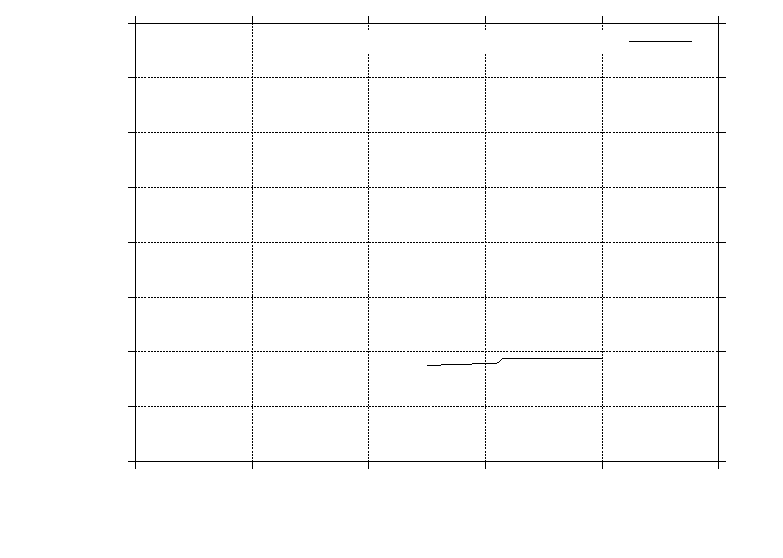
\includegraphics{E0ddepend}}%
    \gplfronttext
  \end{picture}%
\endgroup
  
\caption{The ground state free energy for $T = 0$, $E_0 + 2\mu N_F$, is plotted as a function of the interwire distance $d$. Black dashed: intrawire pairing only. Black dash-dotted: interwire pairing only. In red: $\Delta^{12}_k$ imaginary. In blue: $\Delta^{12}_k$ real. For the free gas: $(E_0 + 2\mu N_F)/\epsilon_{F,0}N_F = 2/3 = 0.667$. Parameters: $(n_Ba_B^3)^{1/3} = 0.01$, $(n_Ba_{BF}^3)^{1/3} = 0.11$, $l_t = 0$, $\frac{m_B}{m_F} = 7/40$, $\frac{n_F}{n_B^{1/3}} = 0.215$, $v_F/c_0 = 0.33$. }  
\label{fig.2wiresE0ddepend}  
\vspace{0.5cm}
% GNUPLOT: LaTeX picture with Postscript
\begingroup
  \makeatletter
  \providecommand\color[2][]{%
    \GenericError{(gnuplot) \space\space\space\@spaces}{%
      Package color not loaded in conjunction with
      terminal option `colourtext'%
    }{See the gnuplot documentation for explanation.%
    }{Either use 'blacktext' in gnuplot or load the package
      color.sty in LaTeX.}%
    \renewcommand\color[2][]{}%
  }%
  \providecommand\includegraphics[2][]{%
    \GenericError{(gnuplot) \space\space\space\@spaces}{%
      Package graphicx or graphics not loaded%
    }{See the gnuplot documentation for explanation.%
    }{The gnuplot epslatex terminal needs graphicx.sty or graphics.sty.}%
    \renewcommand\includegraphics[2][]{}%
  }%
  \providecommand\rotatebox[2]{#2}%
  \@ifundefined{ifGPcolor}{%
    \newif\ifGPcolor
    \GPcolorfalse
  }{}%
  \@ifundefined{ifGPblacktext}{%
    \newif\ifGPblacktext
    \GPblacktexttrue
  }{}%
  % define a \g@addto@macro without @ in the name:
  \let\gplgaddtomacro\g@addto@macro
  % define empty templates for all commands taking text:
  \gdef\gplbacktext{}%
  \gdef\gplfronttext{}%
  \makeatother
  \ifGPblacktext
    % no textcolor at all
    \def\colorrgb#1{}%
    \def\colorgray#1{}%
  \else
    % gray or color?
    \ifGPcolor
      \def\colorrgb#1{\color[rgb]{#1}}%
      \def\colorgray#1{\color[gray]{#1}}%
      \expandafter\def\csname LTw\endcsname{\color{white}}%
      \expandafter\def\csname LTb\endcsname{\color{black}}%
      \expandafter\def\csname LTa\endcsname{\color{black}}%
      \expandafter\def\csname LT0\endcsname{\color[rgb]{1,0,0}}%
      \expandafter\def\csname LT1\endcsname{\color[rgb]{0,1,0}}%
      \expandafter\def\csname LT2\endcsname{\color[rgb]{0,0,1}}%
      \expandafter\def\csname LT3\endcsname{\color[rgb]{1,0,1}}%
      \expandafter\def\csname LT4\endcsname{\color[rgb]{0,1,1}}%
      \expandafter\def\csname LT5\endcsname{\color[rgb]{1,1,0}}%
      \expandafter\def\csname LT6\endcsname{\color[rgb]{0,0,0}}%
      \expandafter\def\csname LT7\endcsname{\color[rgb]{1,0.3,0}}%
      \expandafter\def\csname LT8\endcsname{\color[rgb]{0.5,0.5,0.5}}%
    \else
      % gray
      \def\colorrgb#1{\color{black}}%
      \def\colorgray#1{\color[gray]{#1}}%
      \expandafter\def\csname LTw\endcsname{\color{white}}%
      \expandafter\def\csname LTb\endcsname{\color{black}}%
      \expandafter\def\csname LTa\endcsname{\color{black}}%
      \expandafter\def\csname LT0\endcsname{\color{black}}%
      \expandafter\def\csname LT1\endcsname{\color{black}}%
      \expandafter\def\csname LT2\endcsname{\color{black}}%
      \expandafter\def\csname LT3\endcsname{\color{black}}%
      \expandafter\def\csname LT4\endcsname{\color{black}}%
      \expandafter\def\csname LT5\endcsname{\color{black}}%
      \expandafter\def\csname LT6\endcsname{\color{black}}%
      \expandafter\def\csname LT7\endcsname{\color{black}}%
      \expandafter\def\csname LT8\endcsname{\color{black}}%
    \fi
  \fi
    \setlength{\unitlength}{0.0500bp}%
    \ifx\gptboxheight\undefined%
      \newlength{\gptboxheight}%
      \newlength{\gptboxwidth}%
      \newsavebox{\gptboxtext}%
    \fi%
    \setlength{\fboxrule}{0.5pt}%
    \setlength{\fboxsep}{1pt}%
\begin{picture}(7200.00,5040.00)%
    \gplgaddtomacro\gplbacktext{%
      \csname LTb\endcsname%
      \put(814,767){\makebox(0,0)[r]{\strut{}$0$}}%
      \csname LTb\endcsname%
      \put(814,1469){\makebox(0,0)[r]{\strut{}$0.1$}}%
      \csname LTb\endcsname%
      \put(814,2170){\makebox(0,0)[r]{\strut{}$0.2$}}%
      \csname LTb\endcsname%
      \put(814,2872){\makebox(0,0)[r]{\strut{}$0.3$}}%
      \csname LTb\endcsname%
      \put(814,3573){\makebox(0,0)[r]{\strut{}$0.4$}}%
      \csname LTb\endcsname%
      \put(814,4275){\makebox(0,0)[r]{\strut{}$0.5$}}%
      \csname LTb\endcsname%
      \put(814,4976){\makebox(0,0)[r]{\strut{}$0.6$}}%
      \csname LTb\endcsname%
      \put(1009,484){\makebox(0,0){\strut{}$0.71$}}%
      \csname LTb\endcsname%
      \put(1828,484){\makebox(0,0){\strut{}$0.72$}}%
      \csname LTb\endcsname%
      \put(2646,484){\makebox(0,0){\strut{}$0.73$}}%
      \csname LTb\endcsname%
      \put(3465,484){\makebox(0,0){\strut{}$0.74$}}%
      \csname LTb\endcsname%
      \put(4284,484){\makebox(0,0){\strut{}$0.75$}}%
      \csname LTb\endcsname%
      \put(5103,484){\makebox(0,0){\strut{}$0.76$}}%
      \csname LTb\endcsname%
      \put(5921,484){\makebox(0,0){\strut{}$0.77$}}%
      \csname LTb\endcsname%
      \put(6740,484){\makebox(0,0){\strut{}$0.78$}}%
    }%
    \gplgaddtomacro\gplfronttext{%
      \csname LTb\endcsname%
      \put(176,2871){\rotatebox{-270}{\makebox(0,0){\strut{}$Delta_k/epsilon_{F,0}$}}}%
      \put(3874,154){\makebox(0,0){\strut{}$k_Fd$}}%
      \csname LTb\endcsname%
      \put(3385,4803){\makebox(0,0)[r]{\strut{}$Intrawire pairing$}}%
      \csname LTb\endcsname%
      \put(3385,4583){\makebox(0,0)[r]{\strut{}$Interwire pairing$}}%
    }%
    \gplbacktext
    \put(0,0){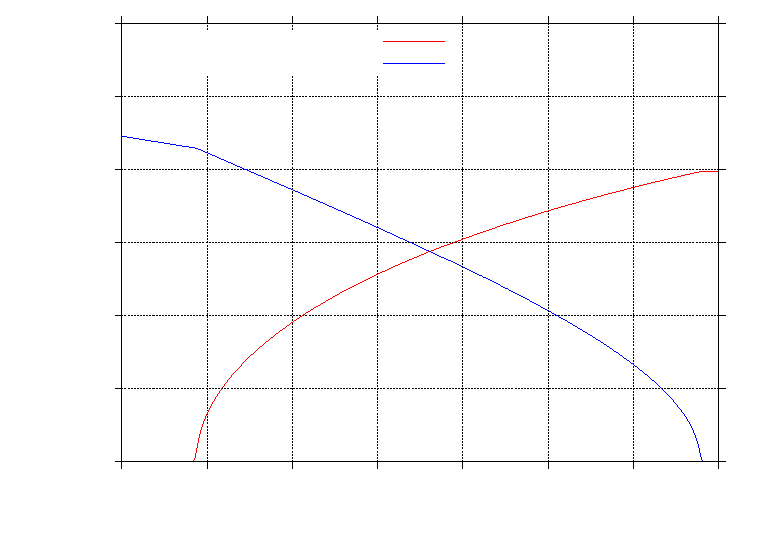
\includegraphics{ddepend}}%
    \gplfronttext
  \end{picture}%
\endgroup
  
\caption{The pairings at the Fermi momentum, $\left|\Delta^{11}_{k_F}\right|$ and $\left|\Delta^{12}_{k_F}\right|$, as a function of the distance $d$ between the wires. In red: pairings for $\Delta^{12}_k$ imaginary, corresponding to the red graph in figure \ref{fig.2wiresE0ddepend}. In blue: Pairings for $\Delta^{12}_k$ real, corresponding to the blue graph in figure \ref{fig.2wiresE0ddepend}. The \textit{inter}wire pairing are shown with dash-dotted lines. The \textit{intra}wire pairings are shown in solid. Parameters: $(n_Ba_B^3)^{1/3} = 0.01$, $(n_Ba_{BF}^3)^{1/3} = 0.11$, $l_t = 0$, $\frac{m_B}{m_F} = 7/40$, $\frac{n_F}{n_B^{1/3}} = 0.215$, $v_F/c_0 = 0.33$. }
\label{fig.2wiresMaximalPairingddepend}
\end{center}
\end{figure}

\begin{figure}
\begin{center}
% GNUPLOT: LaTeX picture with Postscript
\begingroup
  \makeatletter
  \providecommand\color[2][]{%
    \GenericError{(gnuplot) \space\space\space\@spaces}{%
      Package color not loaded in conjunction with
      terminal option `colourtext'%
    }{See the gnuplot documentation for explanation.%
    }{Either use 'blacktext' in gnuplot or load the package
      color.sty in LaTeX.}%
    \renewcommand\color[2][]{}%
  }%
  \providecommand\includegraphics[2][]{%
    \GenericError{(gnuplot) \space\space\space\@spaces}{%
      Package graphicx or graphics not loaded%
    }{See the gnuplot documentation for explanation.%
    }{The gnuplot epslatex terminal needs graphicx.sty or graphics.sty.}%
    \renewcommand\includegraphics[2][]{}%
  }%
  \providecommand\rotatebox[2]{#2}%
  \@ifundefined{ifGPcolor}{%
    \newif\ifGPcolor
    \GPcolorfalse
  }{}%
  \@ifundefined{ifGPblacktext}{%
    \newif\ifGPblacktext
    \GPblacktexttrue
  }{}%
  % define a \g@addto@macro without @ in the name:
  \let\gplgaddtomacro\g@addto@macro
  % define empty templates for all commands taking text:
  \gdef\gplbacktext{}%
  \gdef\gplfronttext{}%
  \makeatother
  \ifGPblacktext
    % no textcolor at all
    \def\colorrgb#1{}%
    \def\colorgray#1{}%
  \else
    % gray or color?
    \ifGPcolor
      \def\colorrgb#1{\color[rgb]{#1}}%
      \def\colorgray#1{\color[gray]{#1}}%
      \expandafter\def\csname LTw\endcsname{\color{white}}%
      \expandafter\def\csname LTb\endcsname{\color{black}}%
      \expandafter\def\csname LTa\endcsname{\color{black}}%
      \expandafter\def\csname LT0\endcsname{\color[rgb]{1,0,0}}%
      \expandafter\def\csname LT1\endcsname{\color[rgb]{0,1,0}}%
      \expandafter\def\csname LT2\endcsname{\color[rgb]{0,0,1}}%
      \expandafter\def\csname LT3\endcsname{\color[rgb]{1,0,1}}%
      \expandafter\def\csname LT4\endcsname{\color[rgb]{0,1,1}}%
      \expandafter\def\csname LT5\endcsname{\color[rgb]{1,1,0}}%
      \expandafter\def\csname LT6\endcsname{\color[rgb]{0,0,0}}%
      \expandafter\def\csname LT7\endcsname{\color[rgb]{1,0.3,0}}%
      \expandafter\def\csname LT8\endcsname{\color[rgb]{0.5,0.5,0.5}}%
    \else
      % gray
      \def\colorrgb#1{\color{black}}%
      \def\colorgray#1{\color[gray]{#1}}%
      \expandafter\def\csname LTw\endcsname{\color{white}}%
      \expandafter\def\csname LTb\endcsname{\color{black}}%
      \expandafter\def\csname LTa\endcsname{\color{black}}%
      \expandafter\def\csname LT0\endcsname{\color{black}}%
      \expandafter\def\csname LT1\endcsname{\color{black}}%
      \expandafter\def\csname LT2\endcsname{\color{black}}%
      \expandafter\def\csname LT3\endcsname{\color{black}}%
      \expandafter\def\csname LT4\endcsname{\color{black}}%
      \expandafter\def\csname LT5\endcsname{\color{black}}%
      \expandafter\def\csname LT6\endcsname{\color{black}}%
      \expandafter\def\csname LT7\endcsname{\color{black}}%
      \expandafter\def\csname LT8\endcsname{\color{black}}%
    \fi
  \fi
    \setlength{\unitlength}{0.0500bp}%
    \ifx\gptboxheight\undefined%
      \newlength{\gptboxheight}%
      \newlength{\gptboxwidth}%
      \newsavebox{\gptboxtext}%
    \fi%
    \setlength{\fboxrule}{0.5pt}%
    \setlength{\fboxsep}{1pt}%
\begin{picture}(7200.00,5040.00)%
    \gplgaddtomacro\gplbacktext{%
      \csname LTb\endcsname%
      \put(814,767){\makebox(0,0)[r]{\strut{}$0$}}%
      \csname LTb\endcsname%
      \put(814,1469){\makebox(0,0)[r]{\strut{}$0.2$}}%
      \csname LTb\endcsname%
      \put(814,2170){\makebox(0,0)[r]{\strut{}$0.4$}}%
      \csname LTb\endcsname%
      \put(814,2872){\makebox(0,0)[r]{\strut{}$0.6$}}%
      \csname LTb\endcsname%
      \put(814,3573){\makebox(0,0)[r]{\strut{}$0.8$}}%
      \csname LTb\endcsname%
      \put(814,4275){\makebox(0,0)[r]{\strut{}$1$}}%
      \csname LTb\endcsname%
      \put(814,4976){\makebox(0,0)[r]{\strut{}$1.2$}}%
      \csname LTb\endcsname%
      \put(1009,484){\makebox(0,0){\strut{}$0.74$}}%
      \csname LTb\endcsname%
      \put(1828,484){\makebox(0,0){\strut{}$0.745$}}%
      \csname LTb\endcsname%
      \put(2646,484){\makebox(0,0){\strut{}$0.75$}}%
      \csname LTb\endcsname%
      \put(3465,484){\makebox(0,0){\strut{}$0.755$}}%
      \csname LTb\endcsname%
      \put(4284,484){\makebox(0,0){\strut{}$0.76$}}%
      \csname LTb\endcsname%
      \put(5103,484){\makebox(0,0){\strut{}$0.765$}}%
      \csname LTb\endcsname%
      \put(5921,484){\makebox(0,0){\strut{}$0.77$}}%
      \csname LTb\endcsname%
      \put(6740,484){\makebox(0,0){\strut{}$0.775$}}%
    }%
    \gplgaddtomacro\gplfronttext{%
      \csname LTb\endcsname%
      \put(176,2871){\rotatebox{-270}{\makebox(0,0){\strut{}$2\text{CS}_{1,1}$}}}%
      \put(3874,154){\makebox(0,0){\strut{}$k_Fd$}}%
      \csname LTb\endcsname%
      \put(3047,4803){\makebox(0,0)[l]{\strut{}Interwire pairing imaginary}}%
      \csname LTb\endcsname%
      \put(3047,4583){\makebox(0,0)[l]{\strut{}Interwire pairing real}}%
    }%
    \gplbacktext
    \put(0,0){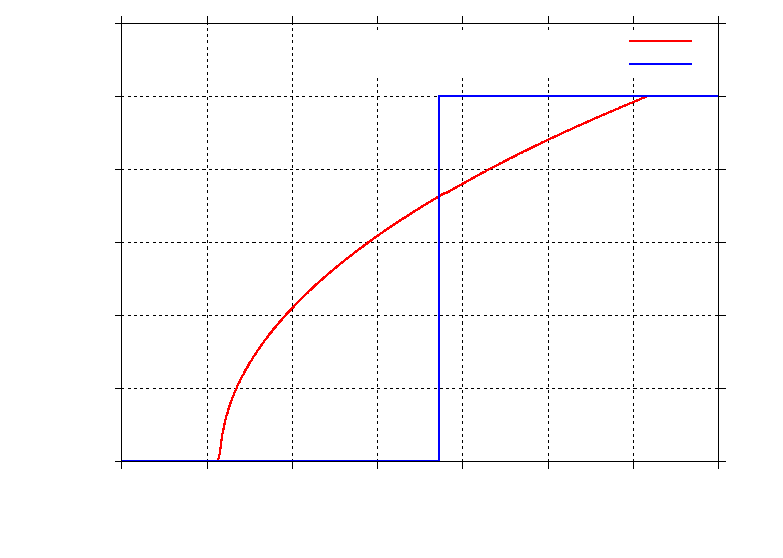
\includegraphics{Figures/twowires/DeltasCS11/CS11depend}}%
    \gplfronttext
  \end{picture}%
\endgroup
  
\caption{The subsystem topological "invariant" $2\text{CS}_{1,1}$. $\text{CS}_{1,2} = - \text{CS}_{1,1}$. In red: $\Delta^{12}_k$ imaginary. For coexistence of $\Delta^{11}_k$ and $\Delta^{12}_k$, $\text{CS}_{1,1}$ is \textit{not} well-defined as an integer invariant. Then it is simply a continuous function, that can take any value. In blue: $\Delta^{12}_k$ real. Parameters: $(n_Ba_B^3)^{1/3} = 0.01$, $(n_Ba_{BF}^3)^{1/3} = 0.11$, $l_t = 0$, $\frac{m_B}{m_F} = 7/40$, $\frac{n_F}{n_B^{1/3}} = 0.215$, $v_F/c_0 = 0.33$. }  
\label{fig.2wiresCS11ddepend}
\end{center}    
\end{figure}

Now let us concentrate on the energetically favourable solution: $\Delta^{12}_k$ imaginary. In this case the energy dispersions are identical and even in $k$: $E^{\pm}_{F,k} = E_{F,k} = \sqrt{\varepsilon_k^2 + (\Delta^{11}_k)^2 + |\Delta^{12}_k|^2}$. This means, that the gap equations in \eqref{eq.2wiresgapequations} partially decouples: 
\begin{align}
\Delta^{11}_k &= -\frac{1}{\mathcal{L}}\sum_{k'} W_{\text{ind}}^{11}(k, k')\frac{\Delta^{11}_{k'}}{2E_{F,k'}}\tanh\left(\frac{\beta E_{F,k'}}{2}\right), \nonumber \\
\Delta^{12}_k &= -\frac{1}{\mathcal{L}}\sum_{k'} W_{\text{ind}}^{12}(k, k')\frac{\Delta^{12}_{k'}}{2E_{F,k'}}\tanh\left(\frac{\beta E_{F,k'}}{2}\right).
\label{eq.2wiresgapequationsDelta12imaginary}
\end{align} 
This explicitly shows, that the two pairings are only coupled through the energy $E_{F,k}$. We start the analysis around $d = d_c$, since both pairings are suspected to be present there. For each value of $d$ we do something very similar to the above. However, here we do not reinitiate the initial guess in each step of $d$. In stead we reuse the found solution from the previous value of $d$. This makes the analysis much faster, and as long as the transition between the pairings is continuous no mistake is made. Further, we record the pairings at the Fermi momentum as above. The result is shown as the red curves in figure \ref{fig.2wiresMaximalPairingddepend}.
 
We see, that for small and large distances the expected behaviour is observed. Naively it seems to be the case, that the interwire pairing increases linearly for small $k_Fd$. However, an analysis to lower values of $d$ shows, that it diverges for $d \to 0$ as expected since the interwire interaction diverges in this limit. In between we see a continuous cross over region, where both pairings are present. Further, we notice that the intrawire pairing is constant from just under $k_Fd = 0.78$ and upwards as we expected. The figure only shows the pairing at $k_F$: $|\Delta_{k_F}|$. We will return to the functional form of the pairings in section \ref{sec.2wirespairingspairwavefunction}.

For clarity we have plotted the subsystem "invariant" $2\text{CS}_{1,1}$ in figure \ref{fig.2wiresCS11ddepend}. In the case of an imaginary interwire pairing, hence only a $T^2 = + \mathbb{I}$ symmetry, we observe the following. For large distances, $k_Fd > 0.8$ for the current set of parameters, only $\Delta^{11}_k$ is present and there is a $T^2 = -\mathbb{I}$ symmetry. Hence, $2\text{CS}_{1,1}$ is a well-defined integer invariant equal to $1$, which is the nontrivial value. For small distances only $\Delta^{12}_k$ is present. Here there is also a $T^2 = -\mathbb{I}$. Again $2\text{CS}_{1,1}$ is a well-defined invariant, now equal to $0$; the trivial value. In-between there is a coexistence of intra- and interwire pairing as already discussed. Then $2\text{CS}_{1,1}$ is not well-defined as an integer invariant, but it is still a continuous function. We also argued for this in the end of subsection \ref{subsec.2wires_CSinv_Delta12imag}. In the case of real interwire pairing the topological invariant flips from $1$ to $0$ at the critical distance $d_c$. 

The combined result of the figures is the following. We are able to find a cross over region of interwire distances $d$, where both an interwire $s$-wave pairing and an intrawire $p$-wave pairing is present, and this transition is the energetically favourable. The continuity of this solution fits with the topological analyses of sections \ref{sec.2wirestransitionqualitative} and \ref{sec.2wires_CSinv}. Further for the imaginary interwire pairing we have not been able to find a continuous transition. The pairing simply flips from $p$- to $s$-wave in a discontinuous manner precisely at $d = d_c$. This is \textit{not} evident from the topological considerations of sections \ref{sec.2wirestransitionqualitative} and \ref{sec.2wires_CSinv}. It is a highly nontrivial numerical result, that the energetically favourable solution is nontopological. This is the main result of the thesis. In the next section we verify, that we have in fact found $p$- and $s$-wave solutions. 


\section{Pairings: Momentum and temperature dependency} \label{sec.2wirespairingspairwavefunction}
In this section we numerically calculate the functional behaviour of the pairings and the pair wave functions for the energetically favourable transition. The analysis is performed in the same manner as in section \ref{sec.2wiresCrossover_energy}. We do not plot the chemical potential, but simply use it to enhance the precision of the pairings.  

We numerically find self-consistent solutions to the above gap equations \eqref{eq.2wiresgapequationsDelta12imaginary} along with the number equation \eqref{eq.2wiresnumberequation}. This is summarized in figure \ref{fig.pairingkdependT0dvaried}. We observe an odd \textit{intra}wire $p$-wave pairing and an even \textit{inter}wire $s$-wave pairing. Further, they show no oscillatory behaviour, they simply decay for large values of $k$. The $p$-wave pairing decays in  a power-law fashion and is well-described by a function on the form $k / (k^2 + a)$. The $s$-wave pairing decays exponentially fast. The overall behaviour of the pairings are seen to be independent of $d$. The interwire pairing is simply enhanced as $d$ decreases, vice versa for the intrawire pairing.  

\begin{figure} 
\begin{center}  
% GNUPLOT: LaTeX picture with Postscript
\begingroup
  \makeatletter
  \providecommand\color[2][]{%
    \GenericError{(gnuplot) \space\space\space\@spaces}{%
      Package color not loaded in conjunction with
      terminal option `colourtext'%
    }{See the gnuplot documentation for explanation.%
    }{Either use 'blacktext' in gnuplot or load the package
      color.sty in LaTeX.}%
    \renewcommand\color[2][]{}%
  }%
  \providecommand\includegraphics[2][]{%
    \GenericError{(gnuplot) \space\space\space\@spaces}{%
      Package graphicx or graphics not loaded%
    }{See the gnuplot documentation for explanation.%
    }{The gnuplot epslatex terminal needs graphicx.sty or graphics.sty.}%
    \renewcommand\includegraphics[2][]{}%
  }%
  \providecommand\rotatebox[2]{#2}%
  \@ifundefined{ifGPcolor}{%
    \newif\ifGPcolor
    \GPcolorfalse
  }{}%
  \@ifundefined{ifGPblacktext}{%
    \newif\ifGPblacktext
    \GPblacktexttrue
  }{}%
  % define a \g@addto@macro without @ in the name:
  \let\gplgaddtomacro\g@addto@macro
  % define empty templates for all commands taking text:
  \gdef\gplbacktext{}%
  \gdef\gplfronttext{}%
  \makeatother
  \ifGPblacktext
    % no textcolor at all
    \def\colorrgb#1{}%
    \def\colorgray#1{}%
  \else
    % gray or color?
    \ifGPcolor
      \def\colorrgb#1{\color[rgb]{#1}}%
      \def\colorgray#1{\color[gray]{#1}}%
      \expandafter\def\csname LTw\endcsname{\color{white}}%
      \expandafter\def\csname LTb\endcsname{\color{black}}%
      \expandafter\def\csname LTa\endcsname{\color{black}}%
      \expandafter\def\csname LT0\endcsname{\color[rgb]{1,0,0}}%
      \expandafter\def\csname LT1\endcsname{\color[rgb]{0,1,0}}%
      \expandafter\def\csname LT2\endcsname{\color[rgb]{0,0,1}}%
      \expandafter\def\csname LT3\endcsname{\color[rgb]{1,0,1}}%
      \expandafter\def\csname LT4\endcsname{\color[rgb]{0,1,1}}%
      \expandafter\def\csname LT5\endcsname{\color[rgb]{1,1,0}}%
      \expandafter\def\csname LT6\endcsname{\color[rgb]{0,0,0}}%
      \expandafter\def\csname LT7\endcsname{\color[rgb]{1,0.3,0}}%
      \expandafter\def\csname LT8\endcsname{\color[rgb]{0.5,0.5,0.5}}%
    \else
      % gray
      \def\colorrgb#1{\color{black}}%
      \def\colorgray#1{\color[gray]{#1}}%
      \expandafter\def\csname LTw\endcsname{\color{white}}%
      \expandafter\def\csname LTb\endcsname{\color{black}}%
      \expandafter\def\csname LTa\endcsname{\color{black}}%
      \expandafter\def\csname LT0\endcsname{\color{black}}%
      \expandafter\def\csname LT1\endcsname{\color{black}}%
      \expandafter\def\csname LT2\endcsname{\color{black}}%
      \expandafter\def\csname LT3\endcsname{\color{black}}%
      \expandafter\def\csname LT4\endcsname{\color{black}}%
      \expandafter\def\csname LT5\endcsname{\color{black}}%
      \expandafter\def\csname LT6\endcsname{\color{black}}%
      \expandafter\def\csname LT7\endcsname{\color{black}}%
      \expandafter\def\csname LT8\endcsname{\color{black}}%
    \fi
  \fi
    \setlength{\unitlength}{0.0500bp}%
    \ifx\gptboxheight\undefined%
      \newlength{\gptboxheight}%
      \newlength{\gptboxwidth}%
      \newsavebox{\gptboxtext}%
    \fi%
    \setlength{\fboxrule}{0.5pt}%
    \setlength{\fboxsep}{1pt}%
\begin{picture}(7200.00,5040.00)%
    \gplgaddtomacro\gplbacktext{%
      \csname LTb\endcsname%
      \put(946,767){\makebox(0,0)[r]{\strut{}$-0.6$}}%
      \csname LTb\endcsname%
      \put(946,1468){\makebox(0,0)[r]{\strut{}$-0.4$}}%
      \csname LTb\endcsname%
      \put(946,2170){\makebox(0,0)[r]{\strut{}$-0.2$}}%
      \csname LTb\endcsname%
      \put(946,2871){\makebox(0,0)[r]{\strut{}$0$}}%
      \csname LTb\endcsname%
      \put(946,3573){\makebox(0,0)[r]{\strut{}$0.2$}}%
      \csname LTb\endcsname%
      \put(946,4275){\makebox(0,0)[r]{\strut{}$0.4$}}%
      \csname LTb\endcsname%
      \put(946,4976){\makebox(0,0)[r]{\strut{}$0.6$}}%
      \csname LTb\endcsname%
      \put(1141,484){\makebox(0,0){\strut{}$-10$}}%
      \csname LTb\endcsname%
      \put(2541,484){\makebox(0,0){\strut{}$-5$}}%
      \csname LTb\endcsname%
      \put(3941,484){\makebox(0,0){\strut{}$0$}}%
      \csname LTb\endcsname%
      \put(5340,484){\makebox(0,0){\strut{}$5$}}%
      \csname LTb\endcsname%
      \put(6740,484){\makebox(0,0){\strut{}$10$}}%
    }%
    \gplgaddtomacro\gplfronttext{%
      \csname LTb\endcsname%
      \put(176,2871){\rotatebox{-270}{\makebox(0,0){\strut{}$\Delta_k/\epsilon_{F,0}$}}}%
      \put(3940,154){\makebox(0,0){\strut{}$k/k_F$}}%
      \csname LTb\endcsname%
      \put(5753,1820){\makebox(0,0)[r]{\strut{}$k_Fd = 0.575$}}%
      \csname LTb\endcsname%
      \put(5753,1600){\makebox(0,0)[r]{\strut{}$k_Fd = 0.585$}}%
      \csname LTb\endcsname%
      \put(5753,1380){\makebox(0,0)[r]{\strut{}$k_Fd = 0.595$}}%
      \csname LTb\endcsname%
      \put(5753,1160){\makebox(0,0)[r]{\strut{}$k_Fd = 0.610$}}%
      \csname LTb\endcsname%
      \put(5753,940){\makebox(0,0)[r]{\strut{}$k_Fd = 0.620$}}%
    }%
    \gplbacktext
    \put(0,0){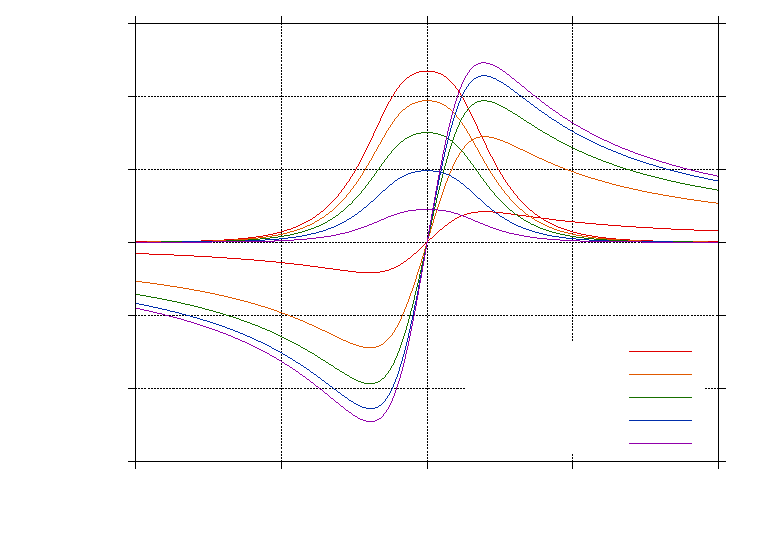
\includegraphics{Figures/twowires/Deltas1/kdepend}}%
    \gplfronttext
  \end{picture}%
\endgroup
  
\caption{The pairings $\Delta^{11}_k$ (odd) and $\Delta^{12}_k$ (even) plotted as a function of $k$ for $\Delta^{12}_k$ imaginary. We see, that the functional behaviour is independent of $d$, and that there is a transition between interwire and intrawire dominated pairing. The intrawire pairing is increased as $d$ increases. Vice versa for the interwire pairing. Parameters: $(n_Ba_B^3)^{1/3} = 0.01$, $(n_Ba_{BF}^3)^{1/3} = 0.11$, $l_t = 0$, $\frac{m_B}{m_F} = 7/40$, $\frac{n_F}{n_B^{1/3}} = 0.215$, $v_F/c_0 = 0.33$. }  
\label{fig.pairingkdependT0dvaried}  
\end{center}    
\end{figure}

Next, we calculate the temperature dependency of the pairings. The expected behaviour can be inferred from the standard BCS-treatment, see e.g. \cite[p. 369]{PlischkeStatPhys}. From here we expect that the pairings have their maximal value for $T = 0$ and decreases monotonically until a critical temperature, $T_c$, is reached. It is however not entirely clear, what effect the presence of two pairings has on this behaviour. 

The result of the analysis for a dominant intrawire pairing is shown in figure \ref{fig.maximalpairingsTdepend_2wires}. We see, that the overall expected behaviour is observed. We observe that the intrawire pairing has a small downward kink, where the interwire pairing vanishes. The same behaviour is seen when the interwire pairing is dominant. This means, that the dominant pairing would be higher at low temperatures if the other pairing was not present: there is a trade off between the size of the individual pairings and the presence of a second pairing.

\begin{figure} 
\begin{center}  
% GNUPLOT: LaTeX picture with Postscript
\begingroup
  \makeatletter
  \providecommand\color[2][]{%
    \GenericError{(gnuplot) \space\space\space\@spaces}{%
      Package color not loaded in conjunction with
      terminal option `colourtext'%
    }{See the gnuplot documentation for explanation.%
    }{Either use 'blacktext' in gnuplot or load the package
      color.sty in LaTeX.}%
    \renewcommand\color[2][]{}%
  }%
  \providecommand\includegraphics[2][]{%
    \GenericError{(gnuplot) \space\space\space\@spaces}{%
      Package graphicx or graphics not loaded%
    }{See the gnuplot documentation for explanation.%
    }{The gnuplot epslatex terminal needs graphicx.sty or graphics.sty.}%
    \renewcommand\includegraphics[2][]{}%
  }%
  \providecommand\rotatebox[2]{#2}%
  \@ifundefined{ifGPcolor}{%
    \newif\ifGPcolor
    \GPcolorfalse
  }{}%
  \@ifundefined{ifGPblacktext}{%
    \newif\ifGPblacktext
    \GPblacktexttrue
  }{}%
  % define a \g@addto@macro without @ in the name:
  \let\gplgaddtomacro\g@addto@macro
  % define empty templates for all commands taking text:
  \gdef\gplbacktext{}%
  \gdef\gplfronttext{}%
  \makeatother
  \ifGPblacktext
    % no textcolor at all
    \def\colorrgb#1{}%
    \def\colorgray#1{}%
  \else
    % gray or color?
    \ifGPcolor
      \def\colorrgb#1{\color[rgb]{#1}}%
      \def\colorgray#1{\color[gray]{#1}}%
      \expandafter\def\csname LTw\endcsname{\color{white}}%
      \expandafter\def\csname LTb\endcsname{\color{black}}%
      \expandafter\def\csname LTa\endcsname{\color{black}}%
      \expandafter\def\csname LT0\endcsname{\color[rgb]{1,0,0}}%
      \expandafter\def\csname LT1\endcsname{\color[rgb]{0,1,0}}%
      \expandafter\def\csname LT2\endcsname{\color[rgb]{0,0,1}}%
      \expandafter\def\csname LT3\endcsname{\color[rgb]{1,0,1}}%
      \expandafter\def\csname LT4\endcsname{\color[rgb]{0,1,1}}%
      \expandafter\def\csname LT5\endcsname{\color[rgb]{1,1,0}}%
      \expandafter\def\csname LT6\endcsname{\color[rgb]{0,0,0}}%
      \expandafter\def\csname LT7\endcsname{\color[rgb]{1,0.3,0}}%
      \expandafter\def\csname LT8\endcsname{\color[rgb]{0.5,0.5,0.5}}%
    \else
      % gray
      \def\colorrgb#1{\color{black}}%
      \def\colorgray#1{\color[gray]{#1}}%
      \expandafter\def\csname LTw\endcsname{\color{white}}%
      \expandafter\def\csname LTb\endcsname{\color{black}}%
      \expandafter\def\csname LTa\endcsname{\color{black}}%
      \expandafter\def\csname LT0\endcsname{\color{black}}%
      \expandafter\def\csname LT1\endcsname{\color{black}}%
      \expandafter\def\csname LT2\endcsname{\color{black}}%
      \expandafter\def\csname LT3\endcsname{\color{black}}%
      \expandafter\def\csname LT4\endcsname{\color{black}}%
      \expandafter\def\csname LT5\endcsname{\color{black}}%
      \expandafter\def\csname LT6\endcsname{\color{black}}%
      \expandafter\def\csname LT7\endcsname{\color{black}}%
      \expandafter\def\csname LT8\endcsname{\color{black}}%
    \fi
  \fi
    \setlength{\unitlength}{0.0500bp}%
    \ifx\gptboxheight\undefined%
      \newlength{\gptboxheight}%
      \newlength{\gptboxwidth}%
      \newsavebox{\gptboxtext}%
    \fi%
    \setlength{\fboxrule}{0.5pt}%
    \setlength{\fboxsep}{1pt}%
\begin{picture}(7200.00,5040.00)%
    \gplgaddtomacro\gplbacktext{%
      \csname LTb\endcsname%
      \put(814,767){\makebox(0,0)[r]{\strut{}$0$}}%
      \csname LTb\endcsname%
      \put(814,1609){\makebox(0,0)[r]{\strut{}$0.1$}}%
      \csname LTb\endcsname%
      \put(814,2451){\makebox(0,0)[r]{\strut{}$0.2$}}%
      \csname LTb\endcsname%
      \put(814,3292){\makebox(0,0)[r]{\strut{}$0.3$}}%
      \csname LTb\endcsname%
      \put(814,4134){\makebox(0,0)[r]{\strut{}$0.4$}}%
      \csname LTb\endcsname%
      \put(814,4976){\makebox(0,0)[r]{\strut{}$0.5$}}%
      \csname LTb\endcsname%
      \put(1009,484){\makebox(0,0){\strut{}$0$}}%
      \csname LTb\endcsname%
      \put(1964,484){\makebox(0,0){\strut{}$0.05$}}%
      \csname LTb\endcsname%
      \put(2919,484){\makebox(0,0){\strut{}$0.1$}}%
      \csname LTb\endcsname%
      \put(3875,484){\makebox(0,0){\strut{}$0.15$}}%
      \csname LTb\endcsname%
      \put(4830,484){\makebox(0,0){\strut{}$0.2$}}%
      \csname LTb\endcsname%
      \put(5785,484){\makebox(0,0){\strut{}$0.25$}}%
      \csname LTb\endcsname%
      \put(6740,484){\makebox(0,0){\strut{}$0.3$}}%
    }%
    \gplgaddtomacro\gplfronttext{%
      \csname LTb\endcsname%
      \put(176,2871){\rotatebox{-270}{\makebox(0,0){\strut{}$\max_k[\Delta_k]/\epsilon_{F,0}$}}}%
      \put(3874,154){\makebox(0,0){\strut{}$T/T_F$}}%
    }%
    \gplbacktext
    \put(0,0){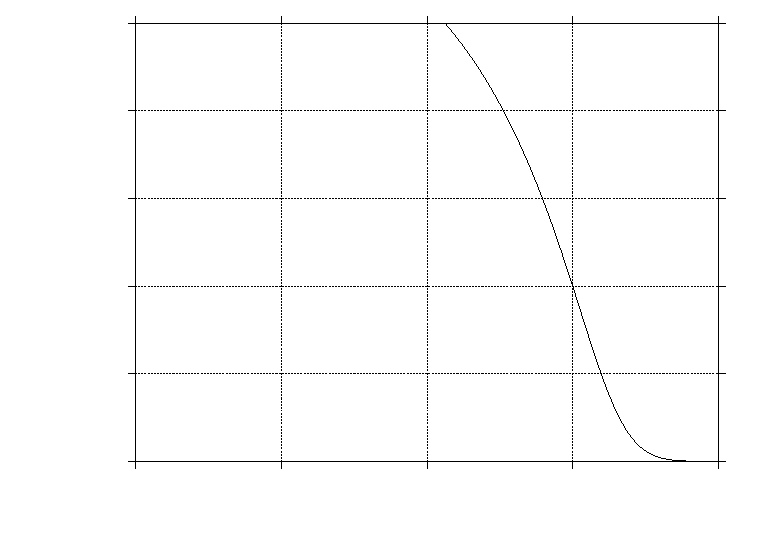
\includegraphics{Figures/twowires/Deltas4.5/Tdepend}}%
    \gplfronttext
  \end{picture}%
\endgroup
  
\caption{Blue solid line: $\max_k[|\Delta^{12}_k|]$ as a function of temperature. Blue dashed line: asymptotic form due to Landau's theory of phase transitions, see equation \eqref{eq.DeltaasymptoteTc}. Red solid line: $\max_k[|\Delta^{11}_k|]$ as a function of temperature. Red dashed line: asymptotic form due to Landau's theory of phase transitions, see equation \eqref{eq.DeltaasymptoteTc}. Notice, that there are two critical temperatures, and that the intrawire pairing shows a downward kink, where the interwire pairing goes to zero. Parameters: $k_Fd = 0.748$, $(n_Ba_B^3)^{1/3} = 0.01$, $(n_Ba_{BF}^3)^{1/3} = 0.11$, $l_t = 0$, $\frac{m_B}{m_F} = 7/40$, $\frac{n_F}{n_B^{1/3}} = 0.215$, $v_F/c_0 = 0.33$.}  
\label{fig.maximalpairingsTdepend_2wires}  
\end{center}    
\end{figure}

The plot shows two phase transitions, one where the \textit{inter}wire pairing goes to zero and one where the \textit{intra}wire pairing goes to zero. These happen at two different critical temperatures, $T^{11}_{c}$ and $T^{12}_{c}$. Near these phase transitions, it is a general result due to Landau, that the order parameter goes as $\sqrt{1 - T/T^{ij}_c}$, see section \ref{sec.landauphasetransitions} and \cite[86-87]{PlischkeStatPhys}. The pairing potentials are linearly dependent on the mean fields, $\braket{c_{i, -k}c_{j,k}}$, which are the order parameters in the present case. Hence, close to the critical temperatures $T^{ij}_c$ we must have:
\begin{equation}
\max_k[\Delta^{ij}_k](T) = \alpha_{ij} \max_k[\Delta^{ij}_k](T = 0) \sqrt{1 - T/T^{ij}_c}. 
\label{eq.DeltaasymptoteTc}
\end{equation}
We fit these functions to the data close to the critical temperatures by adjusting $\alpha_{ij}$. This results in the dashed lines in figure \ref{fig.maximalpairingsTdepend_2wires}. We observe an excellent agreement. 

In conclusion, the presence of a second type of pairing changes the functional dependency on temperature and lowers the dominant pairing. However, the calculated temperature dependency of the pairings are entirely reliable. This is due to the increasing phase fluctuations with increasing temperature. Significant steps beyond our current formalism must be taken to come with more reliable calculations of the temperature dependency. We will not pursue this any further. For an analysis on the critical temperature of the separated wires within our current formalism the reader is referred to appendix \ref{Appendix.criticaltemperature}. 

\section{Pair wave functions} \label{sec.pairwavefunctions}
To get a physically clearer picture of the effect of the pairings we calculate the pair wave functions in real space. These are correlation functions, that describe how two fermions are correlated as a function of there respective positions. Specifically a high absolute value of $\braket{\psi_{i,F}(x')\psi_{j,F}(x)}$ for specific $x$ and $x'$ means, that the fermions have a tendency to be at those positions $x$ and $x'$. This is the reason why we refer to them as pair wave functions. However, caution should be taken, since the correlation functions are not a direct measure of probability. 

We use the Fourier decomposition $\psi_{1,F}(x) = \frac{1}{\sqrt{\mathcal{L}}} \sum_k \text{e}^{ikx} c_{1,k}$ to get an expression for the pair wave functions. For the fermions in wire 1, we get:
\begin{equation}
\braket{\psi_{1,F}(x')\psi_{1,F}(x)} = \frac{1}{\mathcal{L}} \sum_{k,q} \text{e}^{i(kx' + qx)}\braket{c_{1,k}c_{1,q}} = \frac{1}{\mathcal{L}} \sum_{k} \text{e}^{ik(x' - x)}\braket{c_{1,k}c_{1,-k}} = \frac{i}{\mathcal{L}} \sum_{k} \sin\left(k(x' - x)\right)\braket{c_{1,k}c_{1,-k}}. \nonumber 
\end{equation}
Here we first use, that we consider only states, where opposite momenta couples: $q = -k$. Then we use, that the fermionic operators anticommute, so that $c_{1,k}c_{1,-k}$ is odd in $k$. We notice, that it only depends on the difference $x' - x$. We therefore let $x \to 0$ and $x' \to x$. We then insert the mean field of equation \eqref{eq.meanfield11} for $\Delta^{12}_k$ imaginary, and get:
\begin{equation}
\braket{\psi_{1,F}(x)\psi_{1,F}(0)} = - \braket{\psi_{2,F}(x)\psi_{2,F}(0)} = \frac{i}{\mathcal{L}}\sum_k \sin(kx) \frac{\Delta^{11}_k}{2E_{F,k}}\tanh\left[\frac{ \beta E_{F,k} }{2}\right], 
\label{eq.intrawirepairwavefunction}
\end{equation}
The same calculation is carried through for the interwire pair wave function. This gives:
\begin{equation}
\braket{\psi_{1,F}(x)\psi_{2,F}(0)} = \frac{1}{\mathcal{L}}\sum_k \cos(kx) \frac{\Delta^{12}_k}{2E_{F,k}}\tanh\left[\frac{ \beta E_{F,k} }{2}\right].
\label{eq.interwirepairwavefunction}
\end{equation} 
Here we should note, that if $E^\pm_{F,k} \neq E_{F,k}$ then the above pair wave functions will be altered. From this we can infer an overall functional behaviour. Firstly, we see that $\braket{\psi_{1,F}(x)\psi_{1,F}(0)}$ and $\braket{\psi_{1,F}(x)\psi_{2,F}(0)}$ are respectively odd and even in $x$. Further, $\sin(kx)$ and $\cos(kx)$ oscillate more rapidly as a function of $k$ at higher values of $x$. Therefore, we expect the pair wave functions to decay to 0. This is also physically reasonable: fermions macroscopically far apart should not be correlated. 

A high value of $\left|\braket{\psi_{1,F}(x)\psi_{1,F}(0)}\right|$ means, that there is a tendency of two particles in the same wire to have the interparticle distance $x$. Similarly a high value of $\left|\braket{\psi_{1,F}(x)\psi_{2,F}(0)}\right|$ means, that if a fermion in wire 2 is located at $x' = 0$, there is a tendency of a second fermion to be located at the position $x$ in wire 1.  

\begin{figure} 
\begin{center}  
% GNUPLOT: LaTeX picture with Postscript
\begingroup
  \makeatletter
  \providecommand\color[2][]{%
    \GenericError{(gnuplot) \space\space\space\@spaces}{%
      Package color not loaded in conjunction with
      terminal option `colourtext'%
    }{See the gnuplot documentation for explanation.%
    }{Either use 'blacktext' in gnuplot or load the package
      color.sty in LaTeX.}%
    \renewcommand\color[2][]{}%
  }%
  \providecommand\includegraphics[2][]{%
    \GenericError{(gnuplot) \space\space\space\@spaces}{%
      Package graphicx or graphics not loaded%
    }{See the gnuplot documentation for explanation.%
    }{The gnuplot epslatex terminal needs graphicx.sty or graphics.sty.}%
    \renewcommand\includegraphics[2][]{}%
  }%
  \providecommand\rotatebox[2]{#2}%
  \@ifundefined{ifGPcolor}{%
    \newif\ifGPcolor
    \GPcolorfalse
  }{}%
  \@ifundefined{ifGPblacktext}{%
    \newif\ifGPblacktext
    \GPblacktexttrue
  }{}%
  % define a \g@addto@macro without @ in the name:
  \let\gplgaddtomacro\g@addto@macro
  % define empty templates for all commands taking text:
  \gdef\gplbacktext{}%
  \gdef\gplfronttext{}%
  \makeatother
  \ifGPblacktext
    % no textcolor at all
    \def\colorrgb#1{}%
    \def\colorgray#1{}%
  \else
    % gray or color?
    \ifGPcolor
      \def\colorrgb#1{\color[rgb]{#1}}%
      \def\colorgray#1{\color[gray]{#1}}%
      \expandafter\def\csname LTw\endcsname{\color{white}}%
      \expandafter\def\csname LTb\endcsname{\color{black}}%
      \expandafter\def\csname LTa\endcsname{\color{black}}%
      \expandafter\def\csname LT0\endcsname{\color[rgb]{1,0,0}}%
      \expandafter\def\csname LT1\endcsname{\color[rgb]{0,1,0}}%
      \expandafter\def\csname LT2\endcsname{\color[rgb]{0,0,1}}%
      \expandafter\def\csname LT3\endcsname{\color[rgb]{1,0,1}}%
      \expandafter\def\csname LT4\endcsname{\color[rgb]{0,1,1}}%
      \expandafter\def\csname LT5\endcsname{\color[rgb]{1,1,0}}%
      \expandafter\def\csname LT6\endcsname{\color[rgb]{0,0,0}}%
      \expandafter\def\csname LT7\endcsname{\color[rgb]{1,0.3,0}}%
      \expandafter\def\csname LT8\endcsname{\color[rgb]{0.5,0.5,0.5}}%
    \else
      % gray
      \def\colorrgb#1{\color{black}}%
      \def\colorgray#1{\color[gray]{#1}}%
      \expandafter\def\csname LTw\endcsname{\color{white}}%
      \expandafter\def\csname LTb\endcsname{\color{black}}%
      \expandafter\def\csname LTa\endcsname{\color{black}}%
      \expandafter\def\csname LT0\endcsname{\color{black}}%
      \expandafter\def\csname LT1\endcsname{\color{black}}%
      \expandafter\def\csname LT2\endcsname{\color{black}}%
      \expandafter\def\csname LT3\endcsname{\color{black}}%
      \expandafter\def\csname LT4\endcsname{\color{black}}%
      \expandafter\def\csname LT5\endcsname{\color{black}}%
      \expandafter\def\csname LT6\endcsname{\color{black}}%
      \expandafter\def\csname LT7\endcsname{\color{black}}%
      \expandafter\def\csname LT8\endcsname{\color{black}}%
    \fi
  \fi
    \setlength{\unitlength}{0.0500bp}%
    \ifx\gptboxheight\undefined%
      \newlength{\gptboxheight}%
      \newlength{\gptboxwidth}%
      \newsavebox{\gptboxtext}%
    \fi%
    \setlength{\fboxrule}{0.5pt}%
    \setlength{\fboxsep}{1pt}%
\begin{picture}(7200.00,5040.00)%
    \gplgaddtomacro\gplbacktext{%
      \csname LTb\endcsname%
      \put(1078,1118){\makebox(0,0)[r]{\strut{}$-0.15$}}%
      \csname LTb\endcsname%
      \put(1078,1702){\makebox(0,0)[r]{\strut{}$-0.1$}}%
      \csname LTb\endcsname%
      \put(1078,2287){\makebox(0,0)[r]{\strut{}$-0.05$}}%
      \csname LTb\endcsname%
      \put(1078,2872){\makebox(0,0)[r]{\strut{}$0$}}%
      \csname LTb\endcsname%
      \put(1078,3456){\makebox(0,0)[r]{\strut{}$0.05$}}%
      \csname LTb\endcsname%
      \put(1078,4041){\makebox(0,0)[r]{\strut{}$0.1$}}%
      \csname LTb\endcsname%
      \put(1078,4625){\makebox(0,0)[r]{\strut{}$0.15$}}%
      \csname LTb\endcsname%
      \put(1273,484){\makebox(0,0){\strut{}$-20$}}%
      \csname LTb\endcsname%
      \put(1956,484){\makebox(0,0){\strut{}$-15$}}%
      \csname LTb\endcsname%
      \put(2640,484){\makebox(0,0){\strut{}$-10$}}%
      \csname LTb\endcsname%
      \put(3323,484){\makebox(0,0){\strut{}$-5$}}%
      \csname LTb\endcsname%
      \put(4007,484){\makebox(0,0){\strut{}$0$}}%
      \csname LTb\endcsname%
      \put(4690,484){\makebox(0,0){\strut{}$5$}}%
      \csname LTb\endcsname%
      \put(5373,484){\makebox(0,0){\strut{}$10$}}%
      \csname LTb\endcsname%
      \put(6057,484){\makebox(0,0){\strut{}$15$}}%
      \csname LTb\endcsname%
      \put(6740,484){\makebox(0,0){\strut{}$20$}}%
    }%
    \gplgaddtomacro\gplfronttext{%
      \csname LTb\endcsname%
      \put(176,2871){\rotatebox{-270}{\makebox(0,0){\strut{}$Pair wave functions$}}}%
      \put(4006,154){\makebox(0,0){\strut{}$k_Fx$}}%
      \csname LTb\endcsname%
      \put(5753,1820){\makebox(0,0)[r]{\strut{}$k_Fd = 0.720$}}%
      \csname LTb\endcsname%
      \put(5753,1600){\makebox(0,0)[r]{\strut{}$k_Fd = 0.735$}}%
      \csname LTb\endcsname%
      \put(5753,1380){\makebox(0,0)[r]{\strut{}$k_Fd = 0.750$}}%
      \csname LTb\endcsname%
      \put(5753,1160){\makebox(0,0)[r]{\strut{}$k_Fd = 0.765$}}%
      \csname LTb\endcsname%
      \put(5753,940){\makebox(0,0)[r]{\strut{}$k_Fd = 0.775$}}%
    }%
    \gplbacktext
    \put(0,0){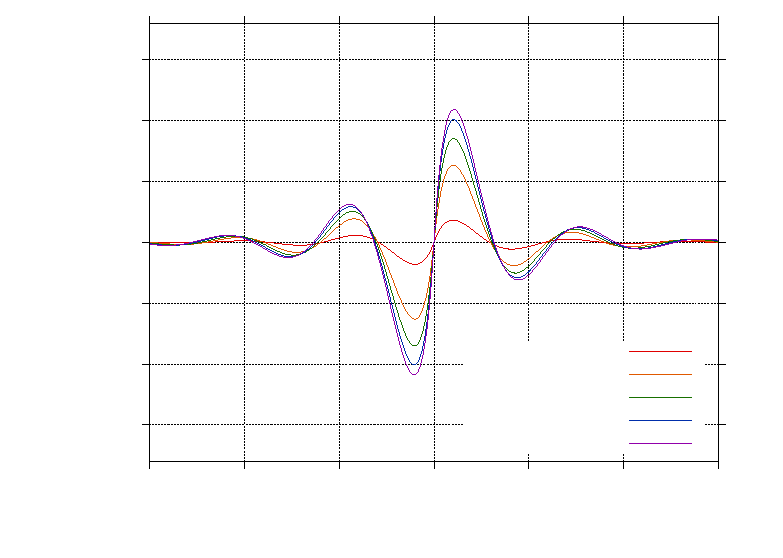
\includegraphics{xdepend11}}%
    \gplfronttext
  \end{picture}%
\endgroup
  
\caption{The \textit{intra}wire pairwave function $\braket{\psi_{1,F}(x)\psi_{1,F}(0)}$ as a function of $x$ for $\Delta^{12}_k$ imaginary. We see, that the functional behaviour is independent of $d$, the pair wave function is simply decreased as $d$ decreases. Parameters: $(n_Ba_B^3)^{1/3} = 0.01$, $(n_Ba_{BF}^3)^{1/3} = 0.11$, $l_t = 0$, $\frac{m_B}{m_F} = 7/40$, $\frac{n_F}{n_B^{1/3}} = 0.215$, $v_F/c_0 = 0.33$. }  
\label{fig.2wirespairwavefunction11}  
\vspace{0.5cm}
% GNUPLOT: LaTeX picture with Postscript
\begingroup
  \makeatletter
  \providecommand\color[2][]{%
    \GenericError{(gnuplot) \space\space\space\@spaces}{%
      Package color not loaded in conjunction with
      terminal option `colourtext'%
    }{See the gnuplot documentation for explanation.%
    }{Either use 'blacktext' in gnuplot or load the package
      color.sty in LaTeX.}%
    \renewcommand\color[2][]{}%
  }%
  \providecommand\includegraphics[2][]{%
    \GenericError{(gnuplot) \space\space\space\@spaces}{%
      Package graphicx or graphics not loaded%
    }{See the gnuplot documentation for explanation.%
    }{The gnuplot epslatex terminal needs graphicx.sty or graphics.sty.}%
    \renewcommand\includegraphics[2][]{}%
  }%
  \providecommand\rotatebox[2]{#2}%
  \@ifundefined{ifGPcolor}{%
    \newif\ifGPcolor
    \GPcolorfalse
  }{}%
  \@ifundefined{ifGPblacktext}{%
    \newif\ifGPblacktext
    \GPblacktexttrue
  }{}%
  % define a \g@addto@macro without @ in the name:
  \let\gplgaddtomacro\g@addto@macro
  % define empty templates for all commands taking text:
  \gdef\gplbacktext{}%
  \gdef\gplfronttext{}%
  \makeatother
  \ifGPblacktext
    % no textcolor at all
    \def\colorrgb#1{}%
    \def\colorgray#1{}%
  \else
    % gray or color?
    \ifGPcolor
      \def\colorrgb#1{\color[rgb]{#1}}%
      \def\colorgray#1{\color[gray]{#1}}%
      \expandafter\def\csname LTw\endcsname{\color{white}}%
      \expandafter\def\csname LTb\endcsname{\color{black}}%
      \expandafter\def\csname LTa\endcsname{\color{black}}%
      \expandafter\def\csname LT0\endcsname{\color[rgb]{1,0,0}}%
      \expandafter\def\csname LT1\endcsname{\color[rgb]{0,1,0}}%
      \expandafter\def\csname LT2\endcsname{\color[rgb]{0,0,1}}%
      \expandafter\def\csname LT3\endcsname{\color[rgb]{1,0,1}}%
      \expandafter\def\csname LT4\endcsname{\color[rgb]{0,1,1}}%
      \expandafter\def\csname LT5\endcsname{\color[rgb]{1,1,0}}%
      \expandafter\def\csname LT6\endcsname{\color[rgb]{0,0,0}}%
      \expandafter\def\csname LT7\endcsname{\color[rgb]{1,0.3,0}}%
      \expandafter\def\csname LT8\endcsname{\color[rgb]{0.5,0.5,0.5}}%
    \else
      % gray
      \def\colorrgb#1{\color{black}}%
      \def\colorgray#1{\color[gray]{#1}}%
      \expandafter\def\csname LTw\endcsname{\color{white}}%
      \expandafter\def\csname LTb\endcsname{\color{black}}%
      \expandafter\def\csname LTa\endcsname{\color{black}}%
      \expandafter\def\csname LT0\endcsname{\color{black}}%
      \expandafter\def\csname LT1\endcsname{\color{black}}%
      \expandafter\def\csname LT2\endcsname{\color{black}}%
      \expandafter\def\csname LT3\endcsname{\color{black}}%
      \expandafter\def\csname LT4\endcsname{\color{black}}%
      \expandafter\def\csname LT5\endcsname{\color{black}}%
      \expandafter\def\csname LT6\endcsname{\color{black}}%
      \expandafter\def\csname LT7\endcsname{\color{black}}%
      \expandafter\def\csname LT8\endcsname{\color{black}}%
    \fi
  \fi
    \setlength{\unitlength}{0.0500bp}%
    \ifx\gptboxheight\undefined%
      \newlength{\gptboxheight}%
      \newlength{\gptboxwidth}%
      \newsavebox{\gptboxtext}%
    \fi%
    \setlength{\fboxrule}{0.5pt}%
    \setlength{\fboxsep}{1pt}%
\begin{picture}(7200.00,5040.00)%
    \gplgaddtomacro\gplbacktext{%
      \csname LTb\endcsname%
      \put(1078,1118){\makebox(0,0)[r]{\strut{}$-0.15$}}%
      \csname LTb\endcsname%
      \put(1078,1702){\makebox(0,0)[r]{\strut{}$-0.1$}}%
      \csname LTb\endcsname%
      \put(1078,2287){\makebox(0,0)[r]{\strut{}$-0.05$}}%
      \csname LTb\endcsname%
      \put(1078,2872){\makebox(0,0)[r]{\strut{}$0$}}%
      \csname LTb\endcsname%
      \put(1078,3456){\makebox(0,0)[r]{\strut{}$0.05$}}%
      \csname LTb\endcsname%
      \put(1078,4041){\makebox(0,0)[r]{\strut{}$0.1$}}%
      \csname LTb\endcsname%
      \put(1078,4625){\makebox(0,0)[r]{\strut{}$0.15$}}%
      \csname LTb\endcsname%
      \put(1273,484){\makebox(0,0){\strut{}$-20$}}%
      \csname LTb\endcsname%
      \put(1956,484){\makebox(0,0){\strut{}$-15$}}%
      \csname LTb\endcsname%
      \put(2640,484){\makebox(0,0){\strut{}$-10$}}%
      \csname LTb\endcsname%
      \put(3323,484){\makebox(0,0){\strut{}$-5$}}%
      \csname LTb\endcsname%
      \put(4007,484){\makebox(0,0){\strut{}$0$}}%
      \csname LTb\endcsname%
      \put(4690,484){\makebox(0,0){\strut{}$5$}}%
      \csname LTb\endcsname%
      \put(5373,484){\makebox(0,0){\strut{}$10$}}%
      \csname LTb\endcsname%
      \put(6057,484){\makebox(0,0){\strut{}$15$}}%
      \csname LTb\endcsname%
      \put(6740,484){\makebox(0,0){\strut{}$20$}}%
    }%
    \gplgaddtomacro\gplfronttext{%
      \csname LTb\endcsname%
      \put(176,2871){\rotatebox{-270}{\makebox(0,0){\strut{}$Pair wave functions$}}}%
      \put(4006,154){\makebox(0,0){\strut{}$k_Fx$}}%
      \csname LTb\endcsname%
      \put(5753,1820){\makebox(0,0)[r]{\strut{}$k_Fd = 0.720$}}%
      \csname LTb\endcsname%
      \put(5753,1600){\makebox(0,0)[r]{\strut{}$k_Fd = 0.735$}}%
      \csname LTb\endcsname%
      \put(5753,1380){\makebox(0,0)[r]{\strut{}$k_Fd = 0.750$}}%
      \csname LTb\endcsname%
      \put(5753,1160){\makebox(0,0)[r]{\strut{}$k_Fd = 0.765$}}%
      \csname LTb\endcsname%
      \put(5753,940){\makebox(0,0)[r]{\strut{}$k_Fd = 0.775$}}%
    }%
    \gplbacktext
    \put(0,0){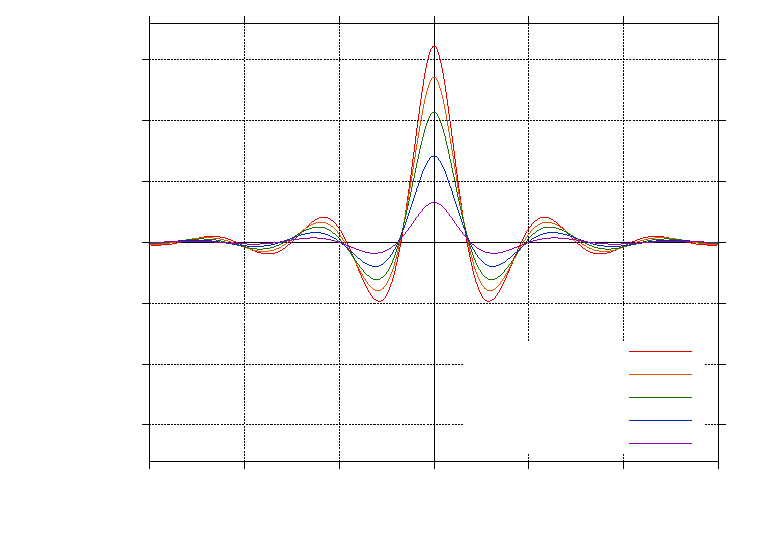
\includegraphics{xdepend12}}%
    \gplfronttext
  \end{picture}%
\endgroup
  
\caption{The \textit{inter}wire pairwave function $\braket{\psi_{1,F}(x)\psi_{2,F}(0)}$ as a function of $x$ for $\Delta^{12}_k$ imaginary. We see, that the functional behaviour is independent of $d$, the pair wave function is simply increased as $d$ decreases. Parameters: $(n_Ba_B^3)^{1/3} = 0.01$, $(n_Ba_{BF}^3)^{1/3} = 0.11$, $l_t = 0$, $\frac{m_B}{m_F} = 7/40$, $\frac{n_F}{n_B^{1/3}} = 0.215$, $v_F/c_0 = 0.33$. }  
\label{fig.2wirespairwavefunction12}  
\end{center}    
\end{figure}

\begin{figure}
\center
\begin{tikzpicture}[scale=2/3]
\pgfmathsetmacro{\hmove}{0}
\pgfmathsetmacro{\distance}{2.5}

\node at (3 + \hmove, 4) {Only intrawire};

\coordinate (a1) at (0.5 + \hmove, 0.14);
\coordinate (a2) at (1.6 + \hmove, 0.14);
\coordinate (a3) at (2.4 + \hmove, 0.14);
\coordinate (correlation) at (3.14, 0);

%Bottom:

\draw[-, thick]  (0 + \hmove, 0) -- (6 + \hmove, 0);
\draw[-|, thick] (0 + \hmove, 0) -- (1 + \hmove, 0);
\draw[-|, thick] (1 + \hmove, 0) -- (2 + \hmove, 0);
\draw[-|, thick] (2 + \hmove, 0) -- (3 + \hmove, 0);
\draw[-|, thick] (3 + \hmove, 0) -- (4 + \hmove, 0);
\draw[-|, thick] (4 + \hmove, 0) -- (5 + \hmove, 0);

\draw[*-, semithick] (a1); 
\draw[*-, semithick] (a1) + (correlation);
%correlation 1:
\coordinate (cor11) at (0.5 - 0.2 + \hmove, 0);
\coordinate (cor12) at (3.14 + 0.5 + 0.2 + \hmove , 0);
\draw[-, thick, red]  (cor11) to[out=90, in=90, distance=0.8cm] (cor12);
\draw[-, thick, red]  (cor11) to[out=-90, in=-90, distance=0.8cm] (cor12);

\draw[*-, semithick] (a2);
\draw[*-, semithick] (a2) + (correlation);
%correlation 2 and 4:
\coordinate (cor21) at (1.6 + 0.2 + \hmove, 0);
\coordinate (prior1) at (0 + \hmove,  0.58);
\coordinate (prior2) at (0 + \hmove, -0.58);

\coordinate (cor22) at (1.6 + 3.14 - 0.2 + \hmove , 0);
\coordinate (post1) at (6 + \hmove,  0.58);
\coordinate (post2) at (6 + \hmove, -0.58);

\draw[-, thick, red]  (cor21) to[out= 90, in=0, distance=0.5cm] (prior1);
\draw[-, thick, red]  (cor21) to[out=-90, in=0, distance=0.5cm] (prior2);

\draw[-, thick, red]  (cor22) to[out= 90, in=180, distance=0.45cm] (post1);
\draw[-, thick, red]  (cor22) to[out=-90, in=180, distance=0.45cm] (post2);

\draw[*-, semithick] (a3);
\draw[*-, semithick] (a3) + (correlation);
%correlation 3:
\coordinate (cor31) at (2.4 - 0.2 + \hmove, 0);
\coordinate (cor32) at (2.4 + 3.14 + 0.2 + \hmove, 0);
\draw[-, thick, red]  (cor31) to[out=90, in=90, distance=0.8cm] (cor32);
\draw[-, thick, red]  (cor31) to[out=-90, in=-90, distance=0.8cm] (cor32);


%Top:
\pgfmathsetmacro{\hmovetoppoints}{-0.2}
\coordinate (a1) at (0.5 + \hmove + \hmovetoppoints, 0.14 + \distance);
\coordinate (a2) at (1.6 + \hmove + \hmovetoppoints, 0.14 + \distance);
\coordinate (a3) at (2.4 + \hmove + \hmovetoppoints, 0.14 + \distance);

\draw[-, thick]  (0 + \hmove, 0 + \distance) -- (6 + \hmove, 0 + \distance);
\draw[-|, thick] (0 + \hmove, 0 + \distance) -- (1 + \hmove, 0 + \distance);
\draw[-|, thick] (1 + \hmove, 0 + \distance) -- (2 + \hmove, 0 + \distance);
\draw[-|, thick] (2 + \hmove, 0 + \distance) -- (3 + \hmove, 0 + \distance);
\draw[-|, thick] (3 + \hmove, 0 + \distance) -- (4 + \hmove, 0 + \distance);
\draw[-|, thick] (4 + \hmove, 0 + \distance) -- (5 + \hmove, 0 + \distance);

\draw[*-, semithick] (a1); 
\draw[*-, semithick] (a1) + (correlation);
%correlation 1:
\coordinate (cor11) at (0.5 - 0.2 + \hmove + \hmovetoppoints, 0 + \distance);
\coordinate (cor12) at (3.14 + 0.5 + 0.2 + \hmove + \hmovetoppoints, 0 + \distance);
\draw[-, thick, red]  (cor11) to[out=90, in=90, distance=0.8cm] (cor12);
\draw[-, thick, red]  (cor11) to[out=-90, in=-90, distance=0.8cm] (cor12);

\draw[*-, semithick] (a2);
\draw[*-, semithick] (a2) + (correlation);
%correlation 2 and 4:
\coordinate (cor21) at (1.6 + 0.2 + \hmove + \hmovetoppoints, 0 + \distance);
\coordinate (prior1) at (0 + \hmove,  0.58 + \distance);
\coordinate (prior2) at (0 + \hmove, -0.58 + \distance);

\coordinate (cor22) at (1.6 + 3.14 - 0.2 + \hmove + \hmovetoppoints , 0 + \distance);
\coordinate (post1) at (6 + \hmove,  0.58 + \distance);
\coordinate (post2) at (6 + \hmove, -0.58 + \distance);

\draw[-, thick, red]  (cor21) to[out= 90, in=0, distance=0.45cm] (prior1);
\draw[-, thick, red]  (cor21) to[out=-90, in=0, distance=0.45cm] (prior2);

\draw[-, thick, red]  (cor22) to[out= 90, in=180, distance=0.5cm] (post1);
\draw[-, thick, red]  (cor22) to[out=-90, in=180, distance=0.5cm] (post2);

\draw[*-, semithick] (a3);
\draw[*-, semithick] (a3) + (correlation);
%correlation 3:
\coordinate (cor31) at (2.4 - 0.2 + \hmove + \hmovetoppoints, 0 + \distance);
\coordinate (cor32) at (2.4 + 3.14 + 0.2 + \hmove + \hmovetoppoints, 0 + \distance);
\draw[-, thick, red]  (cor31) to[out=90, in=90, distance=0.8cm] (cor32);
\draw[-, thick, red]  (cor31) to[out=-90, in=-90, distance=0.8cm] (cor32);

%%%%%%%%%%%%%%%%%%%%%%%%%%%%%%%%
%%%%%%%%%%%%%%%%%%%%%%%%%%%%%%%%
%%%%%%%%%%%%%%%%%%%%%%%%%%%%%%%%

\pgfmathsetmacro{\hmove}{7}
\pgfmathsetmacro{\distance}{2}

\node at (3 + \hmove, 4) {Both};

\coordinate (a1) at (0.5 + \hmove, 0.14);
\coordinate (a2) at (1.6 + \hmove, 0.14);
\coordinate (a3) at (2.4 + \hmove, 0.14);
\coordinate (correlation) at (3.14, 0);

%Bottom:

\draw[-, thick]  (0 + \hmove, 0) -- (6 + \hmove, 0);
\draw[-|, thick] (0 + \hmove, 0) -- (1 + \hmove, 0);
\draw[-|, thick] (1 + \hmove, 0) -- (2 + \hmove, 0);
\draw[-|, thick] (2 + \hmove, 0) -- (3 + \hmove, 0);
\draw[-|, thick] (3 + \hmove, 0) -- (4 + \hmove, 0);
\draw[-|, thick] (4 + \hmove, 0) -- (5 + \hmove, 0);

\draw[*-, semithick] (a1); 
\draw[*-, semithick] (a1) + (correlation);
%correlation 1:
\coordinate (cor11) at (0.5 - 0.2 + \hmove, 0);
\coordinate (cor12) at (3.14 + 0.5 + 0.2 + \hmove , 0);
\draw[-, thick, red]  (cor11) to[out=90, in=90, distance=0.8cm] (cor12);
\draw[-, thick, red]  (cor11) to[out=-90, in=-90, distance=0.8cm] (cor12);

\draw[*-, semithick] (a2);
\draw[*-, semithick] (a2) + (correlation);
%correlation 2 and 4:
\coordinate (cor21) at (1.6 + 0.2 + \hmove, 0);
\coordinate (prior1) at (0 + \hmove,  0.58);
\coordinate (prior2) at (0 + \hmove, -0.58);

\coordinate (cor22) at (1.6 + 3.14 - 0.2 + \hmove , 0);
\coordinate (post1) at (6 + \hmove,  0.58);
\coordinate (post2) at (6 + \hmove, -0.58);

\draw[-, thick, red]  (cor21) to[out= 90, in=0, distance=0.5cm] (prior1);
\draw[-, thick, red]  (cor21) to[out=-90, in=0, distance=0.5cm] (prior2);

\draw[-, thick, red]  (cor22) to[out= 90, in=180, distance=0.45cm] (post1);
\draw[-, thick, red]  (cor22) to[out=-90, in=180, distance=0.45cm] (post2);

\draw[*-, semithick] (a3);
\draw[*-, semithick] (a3) + (correlation);
%correlation 3:
\coordinate (cor31) at (2.4 - 0.2 + \hmove, 0);
\coordinate (cor32) at (2.4 + 3.14 + 0.2 + \hmove, 0);
\draw[-, thick, red]  (cor31) to[out=90, in=90, distance=0.8cm] (cor32);
\draw[-, thick, red]  (cor31) to[out=-90, in=-90, distance=0.8cm] (cor32);


%Top:
\coordinate (a1) at (0.5 + \hmove, 0.14 + \distance);
\coordinate (a2) at (1.6 + \hmove, 0.14 + \distance);
\coordinate (a3) at (2.4 + \hmove, 0.14 + \distance);

\draw[-, thick]  (0 + \hmove, 0 + \distance) -- (6 + \hmove, 0 + \distance);
\draw[-|, thick] (0 + \hmove, 0 + \distance) -- (1 + \hmove, 0 + \distance);
\draw[-|, thick] (1 + \hmove, 0 + \distance) -- (2 + \hmove, 0 + \distance);
\draw[-|, thick] (2 + \hmove, 0 + \distance) -- (3 + \hmove, 0 + \distance);
\draw[-|, thick] (3 + \hmove, 0 + \distance) -- (4 + \hmove, 0 + \distance);
\draw[-|, thick] (4 + \hmove, 0 + \distance) -- (5 + \hmove, 0 + \distance);

\draw[*-, semithick] (a1); 
\draw[*-, semithick] (a1) + (correlation);
%correlation 1:
\coordinate (cor11) at (0.5 - 0.2 + \hmove, 0 + \distance);
\coordinate (cor12) at (3.14 + 0.5 + 0.2 + \hmove , 0 + \distance);
\draw[-, thick, red]  (cor11) to[out=90, in=90, distance=0.8cm] (cor12);
\draw[-, thick, red]  (cor11) to[out=-90, in=-90, distance=0.8cm] (cor12);

\draw[*-, semithick] (a2);
\draw[*-, semithick] (a2) + (correlation);
%correlation 2 and 4:
\coordinate (cor21) at (1.6 + 0.2 + \hmove, 0 + \distance);
\coordinate (prior1) at (0 + \hmove,  0.58 + \distance);
\coordinate (prior2) at (0 + \hmove, -0.58 + \distance);

\coordinate (cor22) at (1.6 + 3.14 - 0.2 + \hmove , 0 + \distance);
\coordinate (post1) at (6 + \hmove,  0.58 + \distance);
\coordinate (post2) at (6 + \hmove, -0.58 + \distance);

\draw[-, thick, red]  (cor21) to[out= 90, in=0, distance=0.5cm] (prior1);
\draw[-, thick, red]  (cor21) to[out=-90, in=0, distance=0.5cm] (prior2);

\draw[-, thick, red]  (cor22) to[out= 90, in=180, distance=0.45cm] (post1);
\draw[-, thick, red]  (cor22) to[out=-90, in=180, distance=0.45cm] (post2);

\draw[*-, semithick] (a3);
\draw[*-, semithick] (a3) + (correlation);
%correlation 3:
\coordinate (cor31) at (2.4 - 0.2 + \hmove, 0 + \distance);
\coordinate (cor32) at (2.4 + 3.14 + 0.2 + \hmove, 0 + \distance);
\draw[-, thick, red]  (cor31) to[out=90, in=90, distance=0.8cm] (cor32);
\draw[-, thick, red]  (cor31) to[out=-90, in=-90, distance=0.8cm] (cor32);

%interwire correlations:

%correlation 1 and 4:
\coordinate (cor11) at (0.5 + \hmove, 0 - 0.2);
\coordinate (cor12) at (0.5 + \hmove, 0 + 0.2 + \distance);
\coordinate (cor13) at (0.5 + 3.14 + \hmove, 0 + 0.2 + \distance);
\draw[-, thick, blue]  (cor11) to[out=0, in=0, distance=0.6cm] (cor12);
\draw[-, thick, blue]  (cor11) to[out=180, in=180, distance=0.6cm] (cor12);

\draw[-, thick, blue]  (cor11) + (correlation) to[out=0, in=0, distance=0.6cm] (cor13);
\draw[-, thick, blue]  (cor11) + (correlation) to[out=180, in=180, distance=0.6cm] (cor13);

%correlation 2:
\coordinate (cor21) at (1.6 + \hmove, 0 - 0.2);
\coordinate (cor22) at (1.6 + \hmove, 0 + 0.2 + \distance);
\draw[-, thick, blue]  (cor21) to[out=0, in=0, distance=0.6cm] (cor22);
\draw[-, thick, blue]  (cor21) to[out=180, in=180, distance=0.6cm] (cor22);

%correlation 3 and 6:
\coordinate (cor31) at (2.4 + \hmove, 0 - 0.2);
\coordinate (cor32) at (2.4 + \hmove, 0 + 0.2 + \distance);
\coordinate (cor33) at (2.4 + 3.14 + \hmove, 0 + 0.2 + \distance);
\draw[-, thick, blue]  (cor31) to[out=0, in=0, distance=0.6cm] (cor32);
\draw[-, thick, blue]  (cor31) to[out=180, in=180, distance=0.6cm] (cor32);

\draw[-, thick, blue]  (cor31) + (correlation) to[out=0, in=0, distance=0.6cm] (cor33);
\draw[-, thick, blue]  (cor31) + (correlation) to[out=180, in=180, distance=0.6cm] (cor33);

%correlation 5:
\coordinate (cor51) at (1.6 + 3.14 + \hmove, 0 - 0.2);
\coordinate (cor52) at (1.6 + 3.14 + \hmove, 0 + 0.2 + \distance);
\draw[-, thick, blue]  (cor51) to[out=0, in=0, distance=0.6cm] (cor52);
\draw[-, thick, blue]  (cor51) to[out=180, in=180, distance=0.6cm] (cor52);

%%%%%%%%%%%%%%%%%%%%%%%%%%%%%%%%
%%%%%%%%%%%%%%%%%%%%%%%%%%%%%%%%
%%%%%%%%%%%%%%%%%%%%%%%%%%%%%%%%

\pgfmathsetmacro{\hmove}{14}
\pgfmathsetmacro{\distance}{1.5}

\node at (3 + \hmove, 4) {Only interwire};

\coordinate (a1) at (0.5 + \hmove, 0.14);
\coordinate (a2) at (1.6 + \hmove, 0.14);
\coordinate (a3) at (2.4 + \hmove, 0.14);
\coordinate (correlation) at (3.14, 0);

%Bottom:

\draw[-, thick]  (0 + \hmove, 0) -- (6 + \hmove, 0);
\draw[-|, thick] (0 + \hmove, 0) -- (1 + \hmove, 0);
\draw[-|, thick] (1 + \hmove, 0) -- (2 + \hmove, 0);
\draw[-|, thick] (2 + \hmove, 0) -- (3 + \hmove, 0);
\draw[-|, thick] (3 + \hmove, 0) -- (4 + \hmove, 0);
\draw[-|, thick] (4 + \hmove, 0) -- (5 + \hmove, 0);

\draw[*-, semithick] (a1); 
\draw[*-, semithick] (a1) + (correlation);
\draw[*-, semithick] (a2);
\draw[*-, semithick] (a2) + (correlation);
\draw[*-, semithick] (a3);
\draw[*-, semithick] (a3) + (correlation);


%Top:
\coordinate (a1) at (0.5 + \hmove, 0.14 + \distance);
\coordinate (a2) at (1.6 + \hmove, 0.14 + \distance);
\coordinate (a3) at (2.4 + \hmove, 0.14 + \distance);

\draw[-, thick]  (0 + \hmove, 0 + \distance) -- (6 + \hmove, 0 + \distance);
\draw[-|, thick] (0 + \hmove, 0 + \distance) -- (1 + \hmove, 0 + \distance);
\draw[-|, thick] (1 + \hmove, 0 + \distance) -- (2 + \hmove, 0 + \distance);
\draw[-|, thick] (2 + \hmove, 0 + \distance) -- (3 + \hmove, 0 + \distance);
\draw[-|, thick] (3 + \hmove, 0 + \distance) -- (4 + \hmove, 0 + \distance);
\draw[-|, thick] (4 + \hmove, 0 + \distance) -- (5 + \hmove, 0 + \distance);

\draw[*-, semithick] (a1); 
\draw[*-, semithick] (a1) + (correlation);
\draw[*-, semithick] (a2);
\draw[*-, semithick] (a2) + (correlation);
\draw[*-, semithick] (a3);
\draw[*-, semithick] (a3) + (correlation);

%interwire correlations:

%correlation 1 and 4:
\coordinate (cor11) at (0.5 + \hmove, 0 - 0.2);
\coordinate (cor12) at (0.5 + \hmove, 0 + 0.2 + \distance);
\coordinate (cor13) at (0.5 + 3.14 + \hmove, 0 + 0.2 + \distance);
\draw[-, thick, blue]  (cor11) to[out=0, in=0, distance=0.6cm] (cor12);
\draw[-, thick, blue]  (cor11) to[out=180, in=180, distance=0.6cm] (cor12);

\draw[-, thick, blue]  (cor11) + (correlation) to[out=0, in=0, distance=0.6cm] (cor13);
\draw[-, thick, blue]  (cor11) + (correlation) to[out=180, in=180, distance=0.6cm] (cor13);

%correlation 2:
\coordinate (cor21) at (1.6 + \hmove, 0 - 0.2);
\coordinate (cor22) at (1.6 + \hmove, 0 + 0.2 + \distance);
\draw[-, thick, blue]  (cor21) to[out=0, in=0, distance=0.6cm] (cor22);
\draw[-, thick, blue]  (cor21) to[out=180, in=180, distance=0.6cm] (cor22);

%correlation 3 and 6:
\coordinate (cor31) at (2.4 + \hmove, 0 - 0.2);
\coordinate (cor32) at (2.4 + \hmove, 0 + 0.2 + \distance);
\coordinate (cor33) at (2.4 + 3.14 + \hmove, 0 + 0.2 + \distance);
\draw[-, thick, blue]  (cor31) to[out=0, in=0, distance=0.6cm] (cor32);
\draw[-, thick, blue]  (cor31) to[out=180, in=180, distance=0.6cm] (cor32);

\draw[-, thick, blue]  (cor31) + (correlation) to[out=0, in=0, distance=0.6cm] (cor33);
\draw[-, thick, blue]  (cor31) + (correlation) to[out=180, in=180, distance=0.6cm] (cor33);

%correlation 5:
\coordinate (cor51) at (1.6 + 3.14 + \hmove, 0 - 0.2);
\coordinate (cor52) at (1.6 + 3.14 + \hmove, 0 + 0.2 + \distance);
\draw[-, thick, blue]  (cor51) to[out=0, in=0, distance=0.6cm] (cor52);
\draw[-, thick, blue]  (cor51) to[out=180, in=180, distance=0.6cm] (cor52);

\end{tikzpicture}
\caption{Spatial distribution of the fermions along the wires. Intrawire and interwire correlations are shown in red and blue respectively. Left: large interwire distances. The fermions correlate internally in each wire only. Middle: intermediate interwire distances. The fermions correlate both internally and across the wires. Right: small interwire distances. The fermions only correlate across the wires.}
\label{fig.2wirespositioncorrelations}
\end{figure}

By using the pairings found in the above analysis we can readily calculate the pair wave functions numerically. The result is shown in figures \ref{fig.2wirespairwavefunction11} and \ref{fig.2wirespairwavefunction12}. They have the following physical interpretation. The \textit{intra}wire pair wave function: fermions correlate over several interparticle distances. The correlation is decreased when we decrease the interwire distance, $d$. The \textit{inter}wire pair wave function: there is a tendency of a fermion in wire 1 to be facing a fermion in wire 2. This correlation is increased as $d$ decreases. 

In figure \ref{fig.2wirespositioncorrelations} we depict these correlations in a pictorial manner. From here it is also evident, that the pairing tend to order the system. In turn the entropy is lowered. 

\section{Occupancy and energy dispersion}
\label{subsec.relevantmomenta.effectiveinteraction}
In this subsection we will briefly study the energy dispersion and the mean occupancy of the $k$'th state. This will in more detail explain, why it is momenta around the Fermi momentum ($k \approx k_F$), that are relevant to understand the influence of the pairing.  

In figures \ref{fig.EnergyDispersion} and \ref{fig.Occupancy} we have plotted the energy dispersion $E_{F,k}$ and occupancy $\braket{c_{1,k}^\dagger c_{1,k}}$ for $T = 0$. This is done for several values of the interwire distance, $d$. Notice that for $T = 0$, the occupancy from equation \eqref{eq.meanoccupancy} shows, that $\braket{c_{1,k}^\dagger c_{1,k}} = \frac{1}{2}\left(1 -  \frac{\varepsilon_k}{E_{F,k}}\right)$. 

\begin{figure} 
\begin{center}  
% GNUPLOT: LaTeX picture with Postscript
\begingroup
  \makeatletter
  \providecommand\color[2][]{%
    \GenericError{(gnuplot) \space\space\space\@spaces}{%
      Package color not loaded in conjunction with
      terminal option `colourtext'%
    }{See the gnuplot documentation for explanation.%
    }{Either use 'blacktext' in gnuplot or load the package
      color.sty in LaTeX.}%
    \renewcommand\color[2][]{}%
  }%
  \providecommand\includegraphics[2][]{%
    \GenericError{(gnuplot) \space\space\space\@spaces}{%
      Package graphicx or graphics not loaded%
    }{See the gnuplot documentation for explanation.%
    }{The gnuplot epslatex terminal needs graphicx.sty or graphics.sty.}%
    \renewcommand\includegraphics[2][]{}%
  }%
  \providecommand\rotatebox[2]{#2}%
  \@ifundefined{ifGPcolor}{%
    \newif\ifGPcolor
    \GPcolortrue
  }{}%
  \@ifundefined{ifGPblacktext}{%
    \newif\ifGPblacktext
    \GPblacktexttrue
  }{}%
  % define a \g@addto@macro without @ in the name:
  \let\gplgaddtomacro\g@addto@macro
  % define empty templates for all commands taking text:
  \gdef\gplbacktext{}%
  \gdef\gplfronttext{}%
  \makeatother
  \ifGPblacktext
    % no textcolor at all
    \def\colorrgb#1{}%
    \def\colorgray#1{}%
  \else
    % gray or color?
    \ifGPcolor
      \def\colorrgb#1{\color[rgb]{#1}}%
      \def\colorgray#1{\color[gray]{#1}}%
      \expandafter\def\csname LTw\endcsname{\color{white}}%
      \expandafter\def\csname LTb\endcsname{\color{black}}%
      \expandafter\def\csname LTa\endcsname{\color{black}}%
      \expandafter\def\csname LT0\endcsname{\color[rgb]{1,0,0}}%
      \expandafter\def\csname LT1\endcsname{\color[rgb]{0,1,0}}%
      \expandafter\def\csname LT2\endcsname{\color[rgb]{0,0,1}}%
      \expandafter\def\csname LT3\endcsname{\color[rgb]{1,0,1}}%
      \expandafter\def\csname LT4\endcsname{\color[rgb]{0,1,1}}%
      \expandafter\def\csname LT5\endcsname{\color[rgb]{1,1,0}}%
      \expandafter\def\csname LT6\endcsname{\color[rgb]{0,0,0}}%
      \expandafter\def\csname LT7\endcsname{\color[rgb]{1,0.3,0}}%
      \expandafter\def\csname LT8\endcsname{\color[rgb]{0.5,0.5,0.5}}%
    \else
      % gray
      \def\colorrgb#1{\color{black}}%
      \def\colorgray#1{\color[gray]{#1}}%
      \expandafter\def\csname LTw\endcsname{\color{white}}%
      \expandafter\def\csname LTb\endcsname{\color{black}}%
      \expandafter\def\csname LTa\endcsname{\color{black}}%
      \expandafter\def\csname LT0\endcsname{\color{black}}%
      \expandafter\def\csname LT1\endcsname{\color{black}}%
      \expandafter\def\csname LT2\endcsname{\color{black}}%
      \expandafter\def\csname LT3\endcsname{\color{black}}%
      \expandafter\def\csname LT4\endcsname{\color{black}}%
      \expandafter\def\csname LT5\endcsname{\color{black}}%
      \expandafter\def\csname LT6\endcsname{\color{black}}%
      \expandafter\def\csname LT7\endcsname{\color{black}}%
      \expandafter\def\csname LT8\endcsname{\color{black}}%
    \fi
  \fi
    \setlength{\unitlength}{0.0500bp}%
    \ifx\gptboxheight\undefined%
      \newlength{\gptboxheight}%
      \newlength{\gptboxwidth}%
      \newsavebox{\gptboxtext}%
    \fi%
    \setlength{\fboxrule}{0.5pt}%
    \setlength{\fboxsep}{1pt}%
\begin{picture}(7200.00,5040.00)%
    \gplgaddtomacro\gplbacktext{%
      \csname LTb\endcsname%
      \put(550,767){\makebox(0,0)[r]{\strut{}$0$}}%
      \csname LTb\endcsname%
      \put(550,1609){\makebox(0,0)[r]{\strut{}$1$}}%
      \csname LTb\endcsname%
      \put(550,2451){\makebox(0,0)[r]{\strut{}$2$}}%
      \csname LTb\endcsname%
      \put(550,3292){\makebox(0,0)[r]{\strut{}$3$}}%
      \csname LTb\endcsname%
      \put(550,4134){\makebox(0,0)[r]{\strut{}$4$}}%
      \csname LTb\endcsname%
      \put(550,4976){\makebox(0,0)[r]{\strut{}$5$}}%
      \csname LTb\endcsname%
      \put(745,484){\makebox(0,0){\strut{}$0$}}%
      \csname LTb\endcsname%
      \put(2244,484){\makebox(0,0){\strut{}$0.5$}}%
      \csname LTb\endcsname%
      \put(3743,484){\makebox(0,0){\strut{}$1$}}%
      \csname LTb\endcsname%
      \put(5241,484){\makebox(0,0){\strut{}$1.5$}}%
      \csname LTb\endcsname%
      \put(6740,484){\makebox(0,0){\strut{}$2$}}%
    }%
    \gplgaddtomacro\gplfronttext{%
      \csname LTb\endcsname%
      \put(176,2871){\rotatebox{-270}{\makebox(0,0){\strut{}$E_{F,k}/\epsilon_{F,0}$}}}%
      \put(3742,154){\makebox(0,0){\strut{}$k/k_F$}}%
      \csname LTb\endcsname%
      \put(4697,4803){\makebox(0,0)[l]{\strut{}Free gas}}%
      \csname LTb\endcsname%
      \put(4697,4583){\makebox(0,0)[l]{\strut{}$k_Fd = 0.70$}}%
      \csname LTb\endcsname%
      \put(4697,4363){\makebox(0,0)[l]{\strut{}$k_Fd = 0.75$}}%
      \csname LTb\endcsname%
      \put(4697,4143){\makebox(0,0)[l]{\strut{}$k_Fd = 0.80$}}%
    }%
    \gplbacktext
    \put(0,0){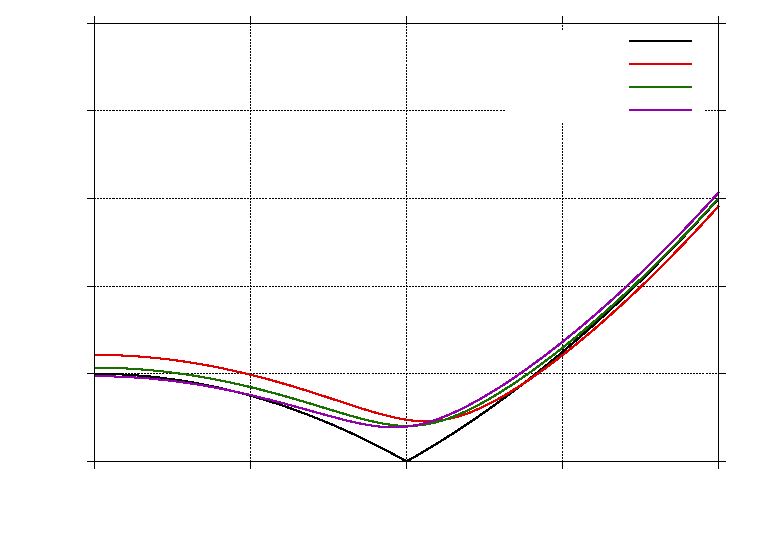
\includegraphics{Figures/twowires/OccupancyT0/energyplot}}%
    \gplfronttext
  \end{picture}%
\endgroup
  
\caption{The energy dispersion is plotted for $T = 0$. Coloured lines: differing values of the relative interparticle distance $n_F / n_B^{1/3}$, superfluid phase. Black line: free gas (normal phase) energy dispersion. The energy is even in $k$, so the graphs are just mirrored for $k < 0$. Parameters: $(n_Ba_B^3)^{1/3} = 0.01$, $(n_Ba_{BF}^3)^{1/3} = 0.11$, $l_t = 0$, $\frac{m_B}{m_F} = 7/40$, $\frac{n_F}{n_B^{1/3}} = 0.215$, $v_F/c_0 = 0.33$. }  
\label{fig.EnergyDispersion}  
\end{center}    
\end{figure}

The energy dispersions are qualitatively similar to the free gas shown in black. The main effect of the pairings are to round off the dispersion at $k \approx k_F$. Further, the value in $k = 0$ is increasingly shifted, with increasin interwire pairing, $\Delta^{12}_k$. This also means, that the occupancy for low $k$-states are lowered, when the interwire pairing increases. This is especially evident from the red curve in figure \ref{fig.Occupancy}. The plots makes it clear, that the relevant momenta for the pairing is around $k = k_F$. 

In our numerical analysis we have noticed, that the chemical potential is shifted \textit{down} for dominant \textit{intra}wire $p$-wave pairing and shifted \textit{up} for \textit{inter}wire $s$-wave pairing. The current analysis illuminates, why this is so. In the intrawire case is most easily understood. The attractive interaction between the wires lowers the energy required to put in an additional fermion, $E$. In turn the chemical potential $\mu = \partial E / \partial N$ is lowered. Superficially this is also true for the \textit{inter}wire interactions. However, here there is the additional effect, that the low-lying $k$-states are partially depleted. Since the chemical potential is the energy at which half the states are occupied, and since som low-lying states are gone, the chemical potential must increase. 

\begin{figure} 
\begin{center}  
% GNUPLOT: LaTeX picture with Postscript
\begingroup
  \makeatletter
  \providecommand\color[2][]{%
    \GenericError{(gnuplot) \space\space\space\@spaces}{%
      Package color not loaded in conjunction with
      terminal option `colourtext'%
    }{See the gnuplot documentation for explanation.%
    }{Either use 'blacktext' in gnuplot or load the package
      color.sty in LaTeX.}%
    \renewcommand\color[2][]{}%
  }%
  \providecommand\includegraphics[2][]{%
    \GenericError{(gnuplot) \space\space\space\@spaces}{%
      Package graphicx or graphics not loaded%
    }{See the gnuplot documentation for explanation.%
    }{The gnuplot epslatex terminal needs graphicx.sty or graphics.sty.}%
    \renewcommand\includegraphics[2][]{}%
  }%
  \providecommand\rotatebox[2]{#2}%
  \@ifundefined{ifGPcolor}{%
    \newif\ifGPcolor
    \GPcolortrue
  }{}%
  \@ifundefined{ifGPblacktext}{%
    \newif\ifGPblacktext
    \GPblacktexttrue
  }{}%
  % define a \g@addto@macro without @ in the name:
  \let\gplgaddtomacro\g@addto@macro
  % define empty templates for all commands taking text:
  \gdef\gplbacktext{}%
  \gdef\gplfronttext{}%
  \makeatother
  \ifGPblacktext
    % no textcolor at all
    \def\colorrgb#1{}%
    \def\colorgray#1{}%
  \else
    % gray or color?
    \ifGPcolor
      \def\colorrgb#1{\color[rgb]{#1}}%
      \def\colorgray#1{\color[gray]{#1}}%
      \expandafter\def\csname LTw\endcsname{\color{white}}%
      \expandafter\def\csname LTb\endcsname{\color{black}}%
      \expandafter\def\csname LTa\endcsname{\color{black}}%
      \expandafter\def\csname LT0\endcsname{\color[rgb]{1,0,0}}%
      \expandafter\def\csname LT1\endcsname{\color[rgb]{0,1,0}}%
      \expandafter\def\csname LT2\endcsname{\color[rgb]{0,0,1}}%
      \expandafter\def\csname LT3\endcsname{\color[rgb]{1,0,1}}%
      \expandafter\def\csname LT4\endcsname{\color[rgb]{0,1,1}}%
      \expandafter\def\csname LT5\endcsname{\color[rgb]{1,1,0}}%
      \expandafter\def\csname LT6\endcsname{\color[rgb]{0,0,0}}%
      \expandafter\def\csname LT7\endcsname{\color[rgb]{1,0.3,0}}%
      \expandafter\def\csname LT8\endcsname{\color[rgb]{0.5,0.5,0.5}}%
    \else
      % gray
      \def\colorrgb#1{\color{black}}%
      \def\colorgray#1{\color[gray]{#1}}%
      \expandafter\def\csname LTw\endcsname{\color{white}}%
      \expandafter\def\csname LTb\endcsname{\color{black}}%
      \expandafter\def\csname LTa\endcsname{\color{black}}%
      \expandafter\def\csname LT0\endcsname{\color{black}}%
      \expandafter\def\csname LT1\endcsname{\color{black}}%
      \expandafter\def\csname LT2\endcsname{\color{black}}%
      \expandafter\def\csname LT3\endcsname{\color{black}}%
      \expandafter\def\csname LT4\endcsname{\color{black}}%
      \expandafter\def\csname LT5\endcsname{\color{black}}%
      \expandafter\def\csname LT6\endcsname{\color{black}}%
      \expandafter\def\csname LT7\endcsname{\color{black}}%
      \expandafter\def\csname LT8\endcsname{\color{black}}%
    \fi
  \fi
    \setlength{\unitlength}{0.0500bp}%
    \ifx\gptboxheight\undefined%
      \newlength{\gptboxheight}%
      \newlength{\gptboxwidth}%
      \newsavebox{\gptboxtext}%
    \fi%
    \setlength{\fboxrule}{0.5pt}%
    \setlength{\fboxsep}{1pt}%
\begin{picture}(7200.00,5040.00)%
    \gplgaddtomacro\gplbacktext{%
      \csname LTb\endcsname%
      \put(814,767){\makebox(0,0)[r]{\strut{}$0$}}%
      \csname LTb\endcsname%
      \put(814,1532){\makebox(0,0)[r]{\strut{}$0.2$}}%
      \csname LTb\endcsname%
      \put(814,2298){\makebox(0,0)[r]{\strut{}$0.4$}}%
      \csname LTb\endcsname%
      \put(814,3063){\makebox(0,0)[r]{\strut{}$0.6$}}%
      \csname LTb\endcsname%
      \put(814,3828){\makebox(0,0)[r]{\strut{}$0.8$}}%
      \csname LTb\endcsname%
      \put(814,4593){\makebox(0,0)[r]{\strut{}$1$}}%
      \csname LTb\endcsname%
      \put(1009,484){\makebox(0,0){\strut{}$0$}}%
      \csname LTb\endcsname%
      \put(2442,484){\makebox(0,0){\strut{}$0.5$}}%
      \csname LTb\endcsname%
      \put(3875,484){\makebox(0,0){\strut{}$1$}}%
      \csname LTb\endcsname%
      \put(5307,484){\makebox(0,0){\strut{}$1.5$}}%
      \csname LTb\endcsname%
      \put(6740,484){\makebox(0,0){\strut{}$2$}}%
    }%
    \gplgaddtomacro\gplfronttext{%
      \csname LTb\endcsname%
      \put(176,2871){\rotatebox{-270}{\makebox(0,0){\strut{}$\braket{c_{1,k}^\dagger c_{1,k}}$}}}%
      \put(3874,154){\makebox(0,0){\strut{}$k/k_F$}}%
      \csname LTb\endcsname%
      \put(4697,4803){\makebox(0,0)[l]{\strut{}Free gas}}%
      \csname LTb\endcsname%
      \put(4697,4583){\makebox(0,0)[l]{\strut{}$k_Fd = 0.70$}}%
      \csname LTb\endcsname%
      \put(4697,4363){\makebox(0,0)[l]{\strut{}$k_Fd = 0.75$}}%
      \csname LTb\endcsname%
      \put(4697,4143){\makebox(0,0)[l]{\strut{}$k_Fd = 0.80$}}%
    }%
    \gplbacktext
    \put(0,0){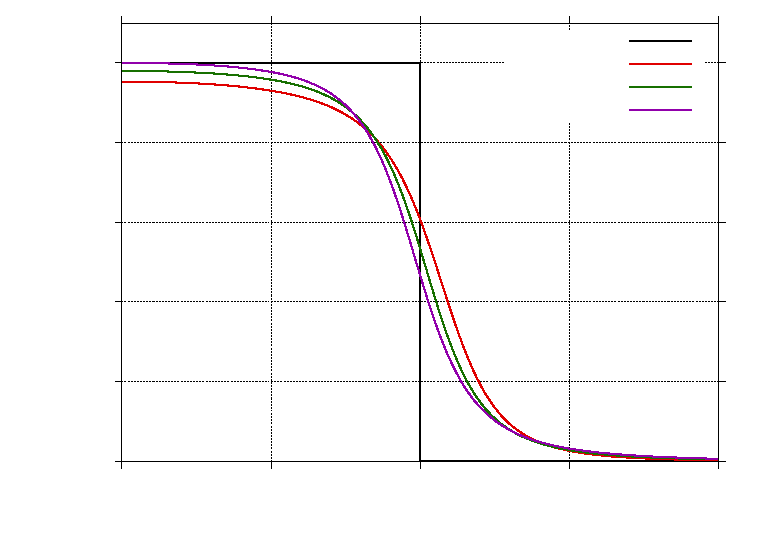
\includegraphics{Figures/twowires/OccupancyT0/Occupancyplot}}%
    \gplfronttext
  \end{picture}%
\endgroup
  
\caption{The number of fermions with momentum $k$, $\braket{c_k^\dagger c_k}$, is plotted for $T = 0$. $\braket{c_k^\dagger c_k} = |v_{F,k}|^2 = \frac{1}{2}\left(1 - \frac{\epsilon_k}{E_{F,k}}\right)$. Coloured lines: differing values of the relative interparticle distance $n_F / n_B^{1/3}$, superfluid phase. Black line: Fermi-Dirac distribution for the free gas (normal phase). Other parameters: Parameters: $(n_Ba_B^3)^{1/3} = 0.01$, $(n_Ba_{BF}^3)^{1/3} = 0.11$, $l_t = 0$, $\frac{m_B}{m_F} = 7/40$, $\frac{n_F}{n_B^{1/3}} = 0.215$, $v_F/c_0 = 0.33$. }  
\label{fig.Occupancy}  
\end{center}    
\end{figure}

In connection with the neglection of retardation effects we already used, that the typical speed of the fermions is the Fermi speed $v_F = k_F/m_F$. The present subsection therefore shows, that this assumption is selfconsistent. This also means, that when we wish to characterize the interactions, we can investigate the effective interactions, $W^{ij}_{\text{ind}}(k, k')$, at the Fermi momentum. Hence, we can set $k = k' = k_F$. We will use this in the following section.


\section{Control of transition through the coherence length}
\label{sec.2wires_crossover_control_coherence_length}
In this section we will investigate how we can control the transition from intrawire to interwire pairing through the coherence length, $\xi$, of the Bose-Einstein condensate. We further investigate the effective interactions at the Fermi momentum, $W^{ij}_{\text{ind}}(k_F, k_F)$, as a function of the coherence length. 

The range of the induced interaction is the condensate coherence length:
\begin{equation}
k_F\frac{\xi}{\sqrt{2}} = \frac{\sqrt{\pi}}{4}\frac{1}{\sqrt{(n_Ba_B^3)^{1/3}}}\frac{n_F}{n_B^{1/3}}.
\label{eq.RangefunctionofrBBnB}
\end{equation}
We would like to explore the possibility of controlling the transition through the coherence length. This is of experimental relevance. Adjusting the spatial distance, $d$, between the wires may be rather difficult in an experimental setup. If we can control an effective distance between the wires by adjusting the coherence length, this then might be a more realisable approach. We have the following intuitive idea of the feasibility of this approach. For a very short coherence length the induced interaction cannot reach across the distance $d$ between the wires. However, there is always a neighbour close by internally in the wire. Hence, we expect that for $\xi \to 0$ the system is in the intrawire pairing only regime. Opposite, for very long coherence lengths the distance between the wires becomes insignificant. Further, since the interwire induced interaction is enhanced by a factor of 2 relative to the intrawire one, we expect that for $\xi \to \infty$ the system enters the interwire pairing only regime. 

The previous section suggests, that we should investigate the effective interactions at the Fermi momentum. We will use the relative particle distance $\frac{n_F}{n_B^{1/3}}$ to vary the coherence length. Hence, we plot $W^{ij}_{\text{ind}}(k_F,k_F)$ as a function of this parameter. This is shown in figure \ref{fig.EffectiveInteraction.nBdepend} for $k_Fd = 0.7$. The overall functional behaviour we understand as follows. When the density of the boson gas increases, the gas becomes increasingly rigid and the fermions have a harder time creating ripples in the gas. Therefore, the effective interactions goes down. The \textit{inter}wire interaction decreases faster, because the interaction has to reach across the interwire distance, $d$. For high values of $\frac{n_F}{n_B^{1/3}}$ on the other hand, the boson gas is depleted, $n_B$ decreases, and there are simply fewer bosons around for the fermions to interact with. Again, the effective interaction goes down. This is in complete accordance with what is seen in an equivalent 2D-3D system studied in the article \cite{BruunZhigangTopSuperfluid}. Further, we notice that in this limit the \textit{inter}wire interaction goes asymptotically to the \textit{intra}wire one. This is because in this limit, the interwire distance becomes insignificant relative to the coherence length, $\xi$. 

\begin{figure} 
\begin{center}  
% GNUPLOT: LaTeX picture with Postscript
\begingroup
  \makeatletter
  \providecommand\color[2][]{%
    \GenericError{(gnuplot) \space\space\space\@spaces}{%
      Package color not loaded in conjunction with
      terminal option `colourtext'%
    }{See the gnuplot documentation for explanation.%
    }{Either use 'blacktext' in gnuplot or load the package
      color.sty in LaTeX.}%
    \renewcommand\color[2][]{}%
  }%
  \providecommand\includegraphics[2][]{%
    \GenericError{(gnuplot) \space\space\space\@spaces}{%
      Package graphicx or graphics not loaded%
    }{See the gnuplot documentation for explanation.%
    }{The gnuplot epslatex terminal needs graphicx.sty or graphics.sty.}%
    \renewcommand\includegraphics[2][]{}%
  }%
  \providecommand\rotatebox[2]{#2}%
  \@ifundefined{ifGPcolor}{%
    \newif\ifGPcolor
    \GPcolortrue
  }{}%
  \@ifundefined{ifGPblacktext}{%
    \newif\ifGPblacktext
    \GPblacktexttrue
  }{}%
  % define a \g@addto@macro without @ in the name:
  \let\gplgaddtomacro\g@addto@macro
  % define empty templates for all commands taking text:
  \gdef\gplbacktext{}%
  \gdef\gplfronttext{}%
  \makeatother
  \ifGPblacktext
    % no textcolor at all
    \def\colorrgb#1{}%
    \def\colorgray#1{}%
  \else
    % gray or color?
    \ifGPcolor
      \def\colorrgb#1{\color[rgb]{#1}}%
      \def\colorgray#1{\color[gray]{#1}}%
      \expandafter\def\csname LTw\endcsname{\color{white}}%
      \expandafter\def\csname LTb\endcsname{\color{black}}%
      \expandafter\def\csname LTa\endcsname{\color{black}}%
      \expandafter\def\csname LT0\endcsname{\color[rgb]{1,0,0}}%
      \expandafter\def\csname LT1\endcsname{\color[rgb]{0,1,0}}%
      \expandafter\def\csname LT2\endcsname{\color[rgb]{0,0,1}}%
      \expandafter\def\csname LT3\endcsname{\color[rgb]{1,0,1}}%
      \expandafter\def\csname LT4\endcsname{\color[rgb]{0,1,1}}%
      \expandafter\def\csname LT5\endcsname{\color[rgb]{1,1,0}}%
      \expandafter\def\csname LT6\endcsname{\color[rgb]{0,0,0}}%
      \expandafter\def\csname LT7\endcsname{\color[rgb]{1,0.3,0}}%
      \expandafter\def\csname LT8\endcsname{\color[rgb]{0.5,0.5,0.5}}%
    \else
      % gray
      \def\colorrgb#1{\color{black}}%
      \def\colorgray#1{\color[gray]{#1}}%
      \expandafter\def\csname LTw\endcsname{\color{white}}%
      \expandafter\def\csname LTb\endcsname{\color{black}}%
      \expandafter\def\csname LTa\endcsname{\color{black}}%
      \expandafter\def\csname LT0\endcsname{\color{black}}%
      \expandafter\def\csname LT1\endcsname{\color{black}}%
      \expandafter\def\csname LT2\endcsname{\color{black}}%
      \expandafter\def\csname LT3\endcsname{\color{black}}%
      \expandafter\def\csname LT4\endcsname{\color{black}}%
      \expandafter\def\csname LT5\endcsname{\color{black}}%
      \expandafter\def\csname LT6\endcsname{\color{black}}%
      \expandafter\def\csname LT7\endcsname{\color{black}}%
      \expandafter\def\csname LT8\endcsname{\color{black}}%
    \fi
  \fi
    \setlength{\unitlength}{0.0500bp}%
    \ifx\gptboxheight\undefined%
      \newlength{\gptboxheight}%
      \newlength{\gptboxwidth}%
      \newsavebox{\gptboxtext}%
    \fi%
    \setlength{\fboxrule}{0.5pt}%
    \setlength{\fboxsep}{1pt}%
\begin{picture}(7200.00,5040.00)%
    \gplgaddtomacro\gplbacktext{%
      \csname LTb\endcsname%
      \put(946,767){\makebox(0,0)[r]{\strut{}$-3$}}%
      \csname LTb\endcsname%
      \put(946,1469){\makebox(0,0)[r]{\strut{}$-2.5$}}%
      \csname LTb\endcsname%
      \put(946,2170){\makebox(0,0)[r]{\strut{}$-2$}}%
      \csname LTb\endcsname%
      \put(946,2872){\makebox(0,0)[r]{\strut{}$-1.5$}}%
      \csname LTb\endcsname%
      \put(946,3573){\makebox(0,0)[r]{\strut{}$-1$}}%
      \csname LTb\endcsname%
      \put(946,4275){\makebox(0,0)[r]{\strut{}$-0.5$}}%
      \csname LTb\endcsname%
      \put(946,4976){\makebox(0,0)[r]{\strut{}$0$}}%
      \csname LTb\endcsname%
      \put(1141,484){\makebox(0,0){\strut{}$0$}}%
      \csname LTb\endcsname%
      \put(1888,484){\makebox(0,0){\strut{}$0.2$}}%
      \csname LTb\endcsname%
      \put(2634,484){\makebox(0,0){\strut{}$0.4$}}%
      \csname LTb\endcsname%
      \put(3381,484){\makebox(0,0){\strut{}$0.6$}}%
      \csname LTb\endcsname%
      \put(4127,484){\makebox(0,0){\strut{}$0.8$}}%
      \csname LTb\endcsname%
      \put(4874,484){\makebox(0,0){\strut{}$1$}}%
      \csname LTb\endcsname%
      \put(5620,484){\makebox(0,0){\strut{}$1.2$}}%
      \csname LTb\endcsname%
      \put(6367,484){\makebox(0,0){\strut{}$1.4$}}%
    }%
    \gplgaddtomacro\gplfronttext{%
      \csname LTb\endcsname%
      \put(176,2871){\rotatebox{-270}{\makebox(0,0){\strut{}$2m_F/k_F W_{\text{ind}}(k_F,k_F)$}}}%
      \put(3940,154){\makebox(0,0){\strut{}$n_F^{1/3}/n_B$}}%
      \csname LTb\endcsname%
      \put(4829,4803){\makebox(0,0)[l]{\strut{}Intrawire}}%
      \csname LTb\endcsname%
      \put(4829,4583){\makebox(0,0)[l]{\strut{}Interwire}}%
    }%
    \gplbacktext
    \put(0,0){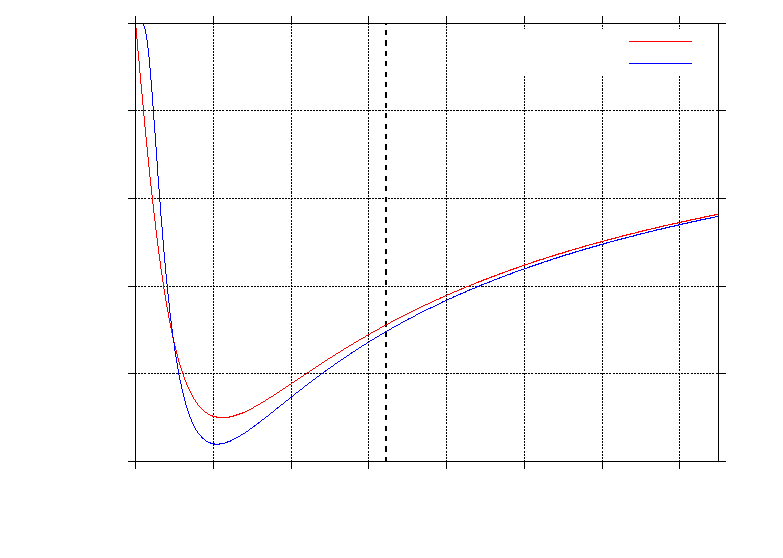
\includegraphics{Figures/twowires/InducedInteraction/InducedInteraction}}%
    \gplfronttext
  \end{picture}%
\endgroup
  
\caption{Solid lines: The effective interactions at the Fermi surface, $W^{ij}_{\text{ind}}(k_F,k_F)$, as a function of relative particle distance $n_F/n_B^{1/3}$. Red line: intrawire effective interaction, $W^{11}_{\text{ind}}(k_F,k_F)$. Blue line: interwire effective interaction, $W^{12}_{\text{ind}}(k_F,k_F)$. Dashed line: indicates where the retardation effects are expected to kick in; the line is made by requiring $v_F/c_0 < 1$. Notice that the effective interactions have an extremal value. Parameters: $k_Fd = 0.7$, $(n_Ba_B^3)^{1/3} = 0.01, (n_Ba_{BF}^3)^{1/3} = 0.1, \frac{m_B}{m_F} = 7/40$.}  
\label{fig.EffectiveInteraction.nBdepend}  
\end{center}    
\end{figure}

We notice, that the \textit{inter}wire interaction becomes dominant around $\frac{n_F}{n_B^{1/3}} = 0.1$. This suggests, that there will be a $p$- to $s$-wave phase transition around this value. Computing whether the intrawire interaction, $W^{11}_{\text{ind}}(k_F,k_F)$, or the interwire interaction, $W^{12}_{\text{ind}}(k_F,k_F)$, is dominant results in the dot-dashed curve in figure \ref{fig.twowirescrossovernBdepend}. 

We now calculate this phase diagram in $d$ and $n_F/n_B^{1/3}$ rigorously. A direct and precise measure for the transition is the previously mentioned critical distance $d_c$. In practice this is found in the following way. First we calculate the free energy $F(\Delta^{11}_k) = E_0(\Delta^{11}_k) + 2 \mu (\Delta^{11}_k) N_F$ in the case, that there is only intrawire pairing, $\Delta^{11}_k$ present. This is independent of $d$ as described by the dashed curve in figure \ref{fig.2wiresE0ddepend}. Then we calculate the same, when only interwire pairing is present. For a constant $n_F/n_B^{1/3}$, we then iteratively find the value of $d = d_c$, where the free energies match: $F(\Delta^{12}_k, d_c) = F(\Delta^{11}_k)$. We then decrease $n_F/n_B^{1/3}$ by a small amount and repeat the process. The outcome of the analysis is shown as the black solid curve in figure \ref{fig.twowirescrossovernBdepend}. We notice, that $d_c$ exhibits a maximal value, and that it approaches a constant for large values of $n_F/n_B^{1/3}$. The dashed vertical line indicates where $v_F = c_0$. To the right of this line retardation effects are expected to kick in. 

The area with white background indicates the \textit{intra}wire pairing only regime. The grey area is correspondingly \textit{inter}wire pairing only. We can understand this result in the following way. First, consider a constant value of the relative particle distance, e.g. $n_F/n_B^{1/3} = 0.2$. When we decrease the interwire distance from say $k_Fd = 1$ we move along the dashed vertical grid line at $n_F/n_B^{1/3} = 0.2$. The system experiences the transition, when we cross the solid black line. This is as described in section \ref{sec.2wiresCrossover_energy}. Second, consider a constant value of the interwire distance, e.g. $k_Fd = 0.6$. When we increase $n_F/n_B^{1/3}$ we follow the horisontal grid line and the system again experiences the transition, when it crosses the solid black line. 

\begin{figure} 
\begin{center}  
% GNUPLOT: LaTeX picture with Postscript
\begingroup
  \makeatletter
  \providecommand\color[2][]{%
    \GenericError{(gnuplot) \space\space\space\@spaces}{%
      Package color not loaded in conjunction with
      terminal option `colourtext'%
    }{See the gnuplot documentation for explanation.%
    }{Either use 'blacktext' in gnuplot or load the package
      color.sty in LaTeX.}%
    \renewcommand\color[2][]{}%
  }%
  \providecommand\includegraphics[2][]{%
    \GenericError{(gnuplot) \space\space\space\@spaces}{%
      Package graphicx or graphics not loaded%
    }{See the gnuplot documentation for explanation.%
    }{The gnuplot epslatex terminal needs graphicx.sty or graphics.sty.}%
    \renewcommand\includegraphics[2][]{}%
  }%
  \providecommand\rotatebox[2]{#2}%
  \@ifundefined{ifGPcolor}{%
    \newif\ifGPcolor
    \GPcolorfalse
  }{}%
  \@ifundefined{ifGPblacktext}{%
    \newif\ifGPblacktext
    \GPblacktexttrue
  }{}%
  % define a \g@addto@macro without @ in the name:
  \let\gplgaddtomacro\g@addto@macro
  % define empty templates for all commands taking text:
  \gdef\gplbacktext{}%
  \gdef\gplfronttext{}%
  \makeatother
  \ifGPblacktext
    % no textcolor at all
    \def\colorrgb#1{}%
    \def\colorgray#1{}%
  \else
    % gray or color?
    \ifGPcolor
      \def\colorrgb#1{\color[rgb]{#1}}%
      \def\colorgray#1{\color[gray]{#1}}%
      \expandafter\def\csname LTw\endcsname{\color{white}}%
      \expandafter\def\csname LTb\endcsname{\color{black}}%
      \expandafter\def\csname LTa\endcsname{\color{black}}%
      \expandafter\def\csname LT0\endcsname{\color[rgb]{1,0,0}}%
      \expandafter\def\csname LT1\endcsname{\color[rgb]{0,1,0}}%
      \expandafter\def\csname LT2\endcsname{\color[rgb]{0,0,1}}%
      \expandafter\def\csname LT3\endcsname{\color[rgb]{1,0,1}}%
      \expandafter\def\csname LT4\endcsname{\color[rgb]{0,1,1}}%
      \expandafter\def\csname LT5\endcsname{\color[rgb]{1,1,0}}%
      \expandafter\def\csname LT6\endcsname{\color[rgb]{0,0,0}}%
      \expandafter\def\csname LT7\endcsname{\color[rgb]{1,0.3,0}}%
      \expandafter\def\csname LT8\endcsname{\color[rgb]{0.5,0.5,0.5}}%
    \else
      % gray
      \def\colorrgb#1{\color{black}}%
      \def\colorgray#1{\color[gray]{#1}}%
      \expandafter\def\csname LTw\endcsname{\color{white}}%
      \expandafter\def\csname LTb\endcsname{\color{black}}%
      \expandafter\def\csname LTa\endcsname{\color{black}}%
      \expandafter\def\csname LT0\endcsname{\color{black}}%
      \expandafter\def\csname LT1\endcsname{\color{black}}%
      \expandafter\def\csname LT2\endcsname{\color{black}}%
      \expandafter\def\csname LT3\endcsname{\color{black}}%
      \expandafter\def\csname LT4\endcsname{\color{black}}%
      \expandafter\def\csname LT5\endcsname{\color{black}}%
      \expandafter\def\csname LT6\endcsname{\color{black}}%
      \expandafter\def\csname LT7\endcsname{\color{black}}%
      \expandafter\def\csname LT8\endcsname{\color{black}}%
    \fi
  \fi
    \setlength{\unitlength}{0.0500bp}%
    \ifx\gptboxheight\undefined%
      \newlength{\gptboxheight}%
      \newlength{\gptboxwidth}%
      \newsavebox{\gptboxtext}%
    \fi%
    \setlength{\fboxrule}{0.5pt}%
    \setlength{\fboxsep}{1pt}%
\begin{picture}(7200.00,5040.00)%
    \gplgaddtomacro\gplbacktext{%
    }%
    \gplgaddtomacro\gplfronttext{%
      \csname LTb\endcsname%
      \put(176,2871){\rotatebox{-270}{\makebox(0,0){\strut{}$k_Fd_c$}}}%
      \put(3874,154){\makebox(0,0){\strut{}$n_F/n_B^{1/3}$}}%
      \csname LTb\endcsname%
      \put(814,767){\makebox(0,0)[r]{\strut{}$0$}}%
      \csname LTb\endcsname%
      \put(814,1469){\makebox(0,0)[r]{\strut{}$0.2$}}%
      \csname LTb\endcsname%
      \put(814,2170){\makebox(0,0)[r]{\strut{}$0.4$}}%
      \csname LTb\endcsname%
      \put(814,2872){\makebox(0,0)[r]{\strut{}$0.6$}}%
      \csname LTb\endcsname%
      \put(814,3573){\makebox(0,0)[r]{\strut{}$0.8$}}%
      \csname LTb\endcsname%
      \put(814,4275){\makebox(0,0)[r]{\strut{}$1$}}%
      \csname LTb\endcsname%
      \put(814,4976){\makebox(0,0)[r]{\strut{}$1.2$}}%
      \csname LTb\endcsname%
      \put(1009,484){\makebox(0,0){\strut{}$0$}}%
      \csname LTb\endcsname%
      \put(1773,484){\makebox(0,0){\strut{}$0.2$}}%
      \csname LTb\endcsname%
      \put(2537,484){\makebox(0,0){\strut{}$0.4$}}%
      \csname LTb\endcsname%
      \put(3301,484){\makebox(0,0){\strut{}$0.6$}}%
      \csname LTb\endcsname%
      \put(4066,484){\makebox(0,0){\strut{}$0.8$}}%
      \csname LTb\endcsname%
      \put(4830,484){\makebox(0,0){\strut{}$1$}}%
      \csname LTb\endcsname%
      \put(5594,484){\makebox(0,0){\strut{}$1.2$}}%
      \csname LTb\endcsname%
      \put(6358,484){\makebox(0,0){\strut{}$1.4$}}%
      \put(1850,3924){\makebox(0,0)[l]{\strut{}Intrawire pairing only}}%
      \put(4142,2521){\makebox(0,0)[l]{\strut{}Interwire pairing only}}%
    }%
    \gplbacktext
    \put(0,0){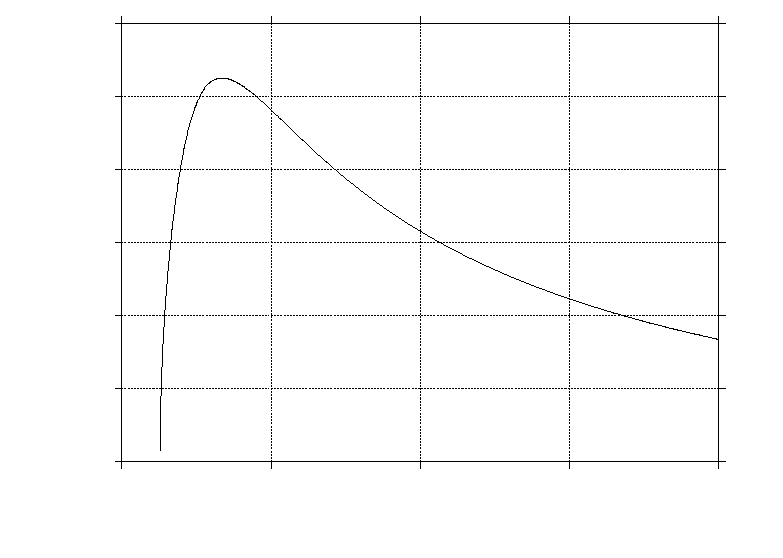
\includegraphics{Figures/twowires/Deltas3.1.3/nBdepend}}%
    \gplfronttext
  \end{picture}%
\endgroup
  
\caption{Solid line: the critical distance $d_c$ plotted as a function of the relative particle distance $n_F/n_B^{1/3}$. White background: intrawire pairing only regime. Grey background: interwire pairing only regime. Dash-dotted line: the critical distance according to the competition of intra- and interwire interactions for $k_Fx_0 = 1/\sqrt{3}$. See equation \eqref{eq.2wires.Vequal}. When we cross the solid line the system experiences the phase transition studied in section \ref{sec.2wiresCrossover_energy}. Dashed vertical line: $v_F = c_0$. Retardation effects are expected to kick in to the right hereof. Parameters: $(n_Ba_B^3)^{1/3} = 0.01$, $(n_Ba_{BF}^3)^{1/3} = 0.11$, $l_t = 0$, $\frac{m_B}{m_F} = 7/40$. }  
\label{fig.twowirescrossovernBdepend}  
\end{center}    
\end{figure}

In this way we explicitly see, that instead of actually moving the wires we can control the transition by adjusting $n_F/n_B^{1/3}$ and in turn the coherence length; see equation \eqref{eq.RangefunctionofrBBnB}. We notice, that the simple analysis based on the effective interactions at the Fermi momentum and the more elaborate but direct calculation of the critical distance $d_c$ are qualitatively similar. However, we notice that the dip in $d_c$ for high values of $n_F/n_B^{1/3}$ is more significant, than the simple analysis suggests. This emphasizes the fact, that although a lot of physical intuition can be build on the form and behaviour of the effective interactions, we have to be careful when used to argue for the response of the system.
